\documentclass[twoside]{book}

% Packages required by doxygen
\usepackage{calc}
\usepackage{doxygen}
\usepackage{graphicx}
\usepackage[utf8]{inputenc}
\usepackage{makeidx}
\usepackage{multicol}
\usepackage{multirow}
\usepackage{textcomp}
\usepackage[table]{xcolor}

% Font selection
\usepackage[T1]{fontenc}
\usepackage{mathptmx}
\usepackage[scaled=.90]{helvet}
\usepackage{courier}
\usepackage{amssymb}
\usepackage{sectsty}
\renewcommand{\familydefault}{\sfdefault}
\allsectionsfont{%
  \fontseries{bc}\selectfont%
  \color{darkgray}%
}
\renewcommand{\DoxyLabelFont}{%
  \fontseries{bc}\selectfont%
  \color{darkgray}%
}

% Page & text layout
\usepackage{geometry}
\geometry{%
  a4paper,%
  top=2.5cm,%
  bottom=2.5cm,%
  left=2.5cm,%
  right=2.5cm%
}
\tolerance=750
\hfuzz=15pt
\hbadness=750
\setlength{\emergencystretch}{15pt}
\setlength{\parindent}{0cm}
\setlength{\parskip}{0.2cm}
\makeatletter
\renewcommand{\paragraph}{%
  \@startsection{paragraph}{4}{0ex}{-1.0ex}{1.0ex}{%
    \normalfont\normalsize\bfseries\SS@parafont%
  }%
}
\renewcommand{\subparagraph}{%
  \@startsection{subparagraph}{5}{0ex}{-1.0ex}{1.0ex}{%
    \normalfont\normalsize\bfseries\SS@subparafont%
  }%
}
\makeatother

% Headers & footers
\usepackage{fancyhdr}
\pagestyle{fancyplain}
\fancyhead[LE]{\fancyplain{}{\bfseries\thepage}}
\fancyhead[CE]{\fancyplain{}{}}
\fancyhead[RE]{\fancyplain{}{\bfseries\leftmark}}
\fancyhead[LO]{\fancyplain{}{\bfseries\rightmark}}
\fancyhead[CO]{\fancyplain{}{}}
\fancyhead[RO]{\fancyplain{}{\bfseries\thepage}}
\fancyfoot[LE]{\fancyplain{}{}}
\fancyfoot[CE]{\fancyplain{}{}}
\fancyfoot[RE]{\fancyplain{}{\bfseries\scriptsize Generated on Thu Apr 30 2015 20\-:23\-:23 for fusion by Doxygen }}
\fancyfoot[LO]{\fancyplain{}{\bfseries\scriptsize Generated on Thu Apr 30 2015 20\-:23\-:23 for fusion by Doxygen }}
\fancyfoot[CO]{\fancyplain{}{}}
\fancyfoot[RO]{\fancyplain{}{}}
\renewcommand{\footrulewidth}{0.4pt}
\renewcommand{\chaptermark}[1]{%
  \markboth{#1}{}%
}
\renewcommand{\sectionmark}[1]{%
  \markright{\thesection\ #1}%
}

% Indices & bibliography
\usepackage{natbib}
\usepackage[titles]{tocloft}
\setcounter{tocdepth}{3}
\setcounter{secnumdepth}{5}
\makeindex

% Hyperlinks (required, but should be loaded last)
\usepackage{ifpdf}
\ifpdf
  \usepackage[pdftex,pagebackref=true]{hyperref}
\else
  \usepackage[ps2pdf,pagebackref=true]{hyperref}
\fi
\hypersetup{%
  colorlinks=true,%
  linkcolor=blue,%
  citecolor=blue,%
  unicode%
}

% Custom commands
\newcommand{\clearemptydoublepage}{%
  \newpage{\pagestyle{empty}\cleardoublepage}%
}


%===== C O N T E N T S =====

\begin{document}

% Titlepage & ToC
\hypersetup{pageanchor=false}
\pagenumbering{roman}
\begin{titlepage}
\vspace*{7cm}
\begin{center}%
{\Large fusion }\\
\vspace*{1cm}
{\large Generated by Doxygen 1.8.6}\\
\vspace*{0.5cm}
{\small Thu Apr 30 2015 20:23:23}\\
\end{center}
\end{titlepage}
\clearemptydoublepage
\tableofcontents
\clearemptydoublepage
\pagenumbering{arabic}
\hypersetup{pageanchor=true}

%--- Begin generated contents ---
\chapter{Namespace Index}
\section{Namespace List}
Here is a list of all namespaces with brief descriptions\-:\begin{DoxyCompactList}
\item\contentsline{section}{\hyperlink{namespace_fusion}{Fusion} }{\pageref{namespace_fusion}}{}
\item\contentsline{section}{\hyperlink{namespace_fusion_1_1_dynamic}{Fusion\-::\-Dynamic} }{\pageref{namespace_fusion_1_1_dynamic}}{}
\item\contentsline{section}{\hyperlink{namespace_fusion_1_1_internal}{Fusion\-::\-Internal} }{\pageref{namespace_fusion_1_1_internal}}{}
\item\contentsline{section}{\hyperlink{namespace_fusion_1_1_static}{Fusion\-::\-Static} }{\pageref{namespace_fusion_1_1_static}}{}
\end{DoxyCompactList}

\chapter{Class Index}
\section{Class List}
Here are the classes, structs, unions and interfaces with brief descriptions\-:\begin{DoxyCompactList}
\item\contentsline{section}{\hyperlink{structbuffer__t}{buffer\-\_\-t} }{\pageref{structbuffer__t}}{}
\item\contentsline{section}{\hyperlink{class_fusion_1_1_dynamic_1_1_dynamic_dispatch}{Fusion\-::\-Dynamic\-::\-Dynamic\-Dispatch$<$ Args $>$} }{\pageref{class_fusion_1_1_dynamic_1_1_dynamic_dispatch}}{}
\item\contentsline{section}{\hyperlink{class_fusion_1_1_static_1_1_static_dispatch}{Fusion\-::\-Static\-::\-Static\-Dispatch$<$ Args $>$} }{\pageref{class_fusion_1_1_static_1_1_static_dispatch}}{}
\end{DoxyCompactList}

\chapter{File Index}
\section{File List}
Here is a list of all files with brief descriptions\-:\begin{DoxyCompactList}
\item\contentsline{section}{\hyperlink{_dynamic_dispatch_8h}{Dynamic\-Dispatch.\-h} }{\pageref{_dynamic_dispatch_8h}}{}
\item\contentsline{section}{\hyperlink{fusion_8h}{fusion.\-h} }{\pageref{fusion_8h}}{}
\item\contentsline{section}{\hyperlink{fusion__info_8h}{fusion\-\_\-info.\-h} }{\pageref{fusion__info_8h}}{}
\item\contentsline{section}{\hyperlink{internal_8h}{internal.\-h} }{\pageref{internal_8h}}{}
\item\contentsline{section}{\hyperlink{_static_dispatch_8h}{Static\-Dispatch.\-h} }{\pageref{_static_dispatch_8h}}{}
\end{DoxyCompactList}

\chapter{Namespace Documentation}
\hypertarget{namespace_fusion}{\section{Fusion Namespace Reference}
\label{namespace_fusion}\index{Fusion@{Fusion}}
}
\subsection*{Namespaces}
\begin{DoxyCompactItemize}
\item 
\hyperlink{namespace_fusion_1_1_dynamic}{Dynamic}
\item 
\hyperlink{namespace_fusion_1_1_internal}{Internal}
\item 
\hyperlink{namespace_fusion_1_1_static}{Static}
\end{DoxyCompactItemize}

\hypertarget{namespace_fusion_1_1_dynamic}{\section{Fusion\-:\-:Dynamic Namespace Reference}
\label{namespace_fusion_1_1_dynamic}\index{Fusion\-::\-Dynamic@{Fusion\-::\-Dynamic}}
}
\subsection*{Classes}
\begin{DoxyCompactItemize}
\item 
class \hyperlink{class_fusion_1_1_dynamic_1_1_dynamic_dispatch}{Dynamic\-Dispatch}
\end{DoxyCompactItemize}
\subsection*{Functions}
\begin{DoxyCompactItemize}
\item 
{\footnotesize template$<$typename... Args$>$ }\\void \hyperlink{namespace_fusion_1_1_dynamic_a152d31c37efe7c83af9d8f899fe80f3e}{work\-Thread} (Args...\-args, function$<$ int(Args..., \hyperlink{structbuffer__t}{buffer\-\_\-t} $\ast$, \hyperlink{structbuffer__t}{buffer\-\_\-t} $\ast$)$>$ func, \hyperlink{structbuffer__t}{buffer\-\_\-t} $\ast$input, \hyperlink{structbuffer__t}{buffer\-\_\-t} $\ast$output, \hyperlink{fusion__info_8h_a015eb90e0de9f16e87bd149d4b9ce959}{status} table\mbox{[}$\,$\mbox{]}, int offset, mutex $\ast$table\-\_\-mutex)
\end{DoxyCompactItemize}


\subsection{Function Documentation}
\hypertarget{namespace_fusion_1_1_dynamic_a152d31c37efe7c83af9d8f899fe80f3e}{\index{Fusion\-::\-Dynamic@{Fusion\-::\-Dynamic}!work\-Thread@{work\-Thread}}
\index{work\-Thread@{work\-Thread}!Fusion::Dynamic@{Fusion\-::\-Dynamic}}
\subsubsection[{work\-Thread}]{\setlength{\rightskip}{0pt plus 5cm}template$<$typename... Args$>$ void Fusion\-::\-Dynamic\-::work\-Thread (
\begin{DoxyParamCaption}
\item[{Args...}]{args, }
\item[{function$<$ int(Args..., {\bf buffer\-\_\-t} $\ast$, {\bf buffer\-\_\-t} $\ast$)$>$}]{func, }
\item[{{\bf buffer\-\_\-t} $\ast$}]{input, }
\item[{{\bf buffer\-\_\-t} $\ast$}]{output, }
\item[{{\bf status}}]{table\mbox{[}$\,$\mbox{]}, }
\item[{int}]{offset, }
\item[{mutex $\ast$}]{table\-\_\-mutex}
\end{DoxyParamCaption}
)}}\label{namespace_fusion_1_1_dynamic_a152d31c37efe7c83af9d8f899fe80f3e}
T\-O\-D\-O\-:find out a way to interrupt cpu work thread 

Here is the call graph for this function\-:
\nopagebreak
\begin{figure}[H]
\begin{center}
\leavevmode
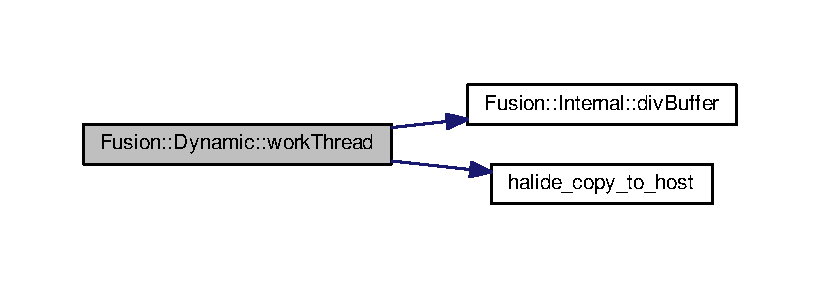
\includegraphics[width=350pt]{namespace_fusion_1_1_dynamic_a152d31c37efe7c83af9d8f899fe80f3e_cgraph}
\end{center}
\end{figure}



\hypertarget{namespace_fusion_1_1_internal}{\section{Fusion\-:\-:Internal Namespace Reference}
\label{namespace_fusion_1_1_internal}\index{Fusion\-::\-Internal@{Fusion\-::\-Internal}}
}
\subsection*{Functions}
\begin{DoxyCompactItemize}
\item 
\hyperlink{structbuffer__t}{buffer\-\_\-t} $\ast$ \hyperlink{namespace_fusion_1_1_internal_afa225bde679af6d7984014f0138aa97d}{div\-Buffer} (\hyperlink{structbuffer__t}{buffer\-\_\-t} $\ast$buf, int start, int nend)
\item 
uint8\-\_\-t $\ast$ \hyperlink{namespace_fusion_1_1_internal_a6e60ee6f87aefcec5b810c52ec9d4abb}{init\-Buffer\-\_\-t} (int x, int y, int z, int w, \hyperlink{structbuffer__t}{buffer\-\_\-t} $\ast$buf, int bit\-Of\-Input)
\end{DoxyCompactItemize}


\subsection{Function Documentation}
\hypertarget{namespace_fusion_1_1_internal_afa225bde679af6d7984014f0138aa97d}{\index{Fusion\-::\-Internal@{Fusion\-::\-Internal}!div\-Buffer@{div\-Buffer}}
\index{div\-Buffer@{div\-Buffer}!Fusion::Internal@{Fusion\-::\-Internal}}
\subsubsection[{div\-Buffer}]{\setlength{\rightskip}{0pt plus 5cm}{\bf buffer\-\_\-t}$\ast$ Fusion\-::\-Internal\-::div\-Buffer (
\begin{DoxyParamCaption}
\item[{{\bf buffer\-\_\-t} $\ast$}]{buf, }
\item[{int}]{start, }
\item[{int}]{nend}
\end{DoxyParamCaption}
)}}\label{namespace_fusion_1_1_internal_afa225bde679af6d7984014f0138aa97d}
\hypertarget{namespace_fusion_1_1_internal_a6e60ee6f87aefcec5b810c52ec9d4abb}{\index{Fusion\-::\-Internal@{Fusion\-::\-Internal}!init\-Buffer\-\_\-t@{init\-Buffer\-\_\-t}}
\index{init\-Buffer\-\_\-t@{init\-Buffer\-\_\-t}!Fusion::Internal@{Fusion\-::\-Internal}}
\subsubsection[{init\-Buffer\-\_\-t}]{\setlength{\rightskip}{0pt plus 5cm}uint8\-\_\-t$\ast$ Fusion\-::\-Internal\-::init\-Buffer\-\_\-t (
\begin{DoxyParamCaption}
\item[{int}]{x, }
\item[{int}]{y, }
\item[{int}]{z, }
\item[{int}]{w, }
\item[{{\bf buffer\-\_\-t} $\ast$}]{buf, }
\item[{int}]{bit\-Of\-Input}
\end{DoxyParamCaption}
)}}\label{namespace_fusion_1_1_internal_a6e60ee6f87aefcec5b810c52ec9d4abb}

\hypertarget{namespace_fusion_1_1_static}{\section{Fusion\-:\-:Static Namespace Reference}
\label{namespace_fusion_1_1_static}\index{Fusion\-::\-Static@{Fusion\-::\-Static}}
}
\subsection*{Classes}
\begin{DoxyCompactItemize}
\item 
class \hyperlink{class_fusion_1_1_static_1_1_static_dispatch}{Static\-Dispatch}
\end{DoxyCompactItemize}
\subsection*{Functions}
\begin{DoxyCompactItemize}
\item 
{\footnotesize template$<$typename... Args$>$ }\\void \hyperlink{namespace_fusion_1_1_static_a4dda28311f1977091df5d7adb5aec742}{gpu\-Stealing} (Args...\-args, function$<$ int(Args..., \hyperlink{structbuffer__t}{buffer\-\_\-t} $\ast$, \hyperlink{structbuffer__t}{buffer\-\_\-t} $\ast$)$>$ func, \hyperlink{structbuffer__t}{buffer\-\_\-t} $\ast$input, \hyperlink{structbuffer__t}{buffer\-\_\-t} $\ast$cpu\-Buf, \hyperlink{structbuffer__t}{buffer\-\_\-t} $\ast$gpu\-Buf, \hyperlink{fusion__info_8h_a015eb90e0de9f16e87bd149d4b9ce959}{status} table\mbox{[}$\,$\mbox{]}, int offset, mutex $\ast$table\-\_\-mutex)
\begin{DoxyCompactList}\small\item\em This Function is a thread function for \hyperlink{namespace_fusion_1_1_static}{Static} execution way with Stealing. \end{DoxyCompactList}\item 
{\footnotesize template$<$typename... Args$>$ }\\void \hyperlink{namespace_fusion_1_1_static_a36302361627ccb126b6aeb0efa6d3ab2}{gpu\-Thread} (Args...\-args, function$<$ int(Args..., \hyperlink{structbuffer__t}{buffer\-\_\-t} $\ast$, \hyperlink{structbuffer__t}{buffer\-\_\-t} $\ast$)$>$ func, \hyperlink{structbuffer__t}{buffer\-\_\-t} $\ast$input, \hyperlink{structbuffer__t}{buffer\-\_\-t} $\ast$output)
\end{DoxyCompactItemize}


\subsection{Function Documentation}
\hypertarget{namespace_fusion_1_1_static_a4dda28311f1977091df5d7adb5aec742}{\index{Fusion\-::\-Static@{Fusion\-::\-Static}!gpu\-Stealing@{gpu\-Stealing}}
\index{gpu\-Stealing@{gpu\-Stealing}!Fusion::Static@{Fusion\-::\-Static}}
\subsubsection[{gpu\-Stealing}]{\setlength{\rightskip}{0pt plus 5cm}template$<$typename... Args$>$ void Fusion\-::\-Static\-::gpu\-Stealing (
\begin{DoxyParamCaption}
\item[{Args...}]{args, }
\item[{function$<$ int(Args..., {\bf buffer\-\_\-t} $\ast$, {\bf buffer\-\_\-t} $\ast$)$>$}]{func, }
\item[{{\bf buffer\-\_\-t} $\ast$}]{input, }
\item[{{\bf buffer\-\_\-t} $\ast$}]{cpu\-Buf, }
\item[{{\bf buffer\-\_\-t} $\ast$}]{gpu\-Buf, }
\item[{{\bf status}}]{table\mbox{[}$\,$\mbox{]}, }
\item[{int}]{offset, }
\item[{mutex $\ast$}]{table\-\_\-mutex}
\end{DoxyParamCaption}
)}}\label{namespace_fusion_1_1_static_a4dda28311f1977091df5d7adb5aec742}


This Function is a thread function for \hyperlink{namespace_fusion_1_1_static}{Static} execution way with Stealing. 


\begin{DoxyParams}{Parameters}
{\em args} & Args arguments for Halide function. \\
\hline
{\em func} & function$<$int(\-Args...,buffer\-\_\-t$\ast$,buffer\-\_\-t$\ast$)$>$ Halide function \\
\hline
\end{DoxyParams}
\begin{DoxyReturn}{Returns}
null
\end{DoxyReturn}
This Function is a thread function for \hyperlink{namespace_fusion_1_1_static}{Static} execution way with Stealing. G\-P\-U will execute the target workload first.\-After that ,G\-P\-U will check the table, if there are still blocks which have not been execute, G\-P\-U will help to execute the block. 

Here is the call graph for this function\-:
\nopagebreak
\begin{figure}[H]
\begin{center}
\leavevmode
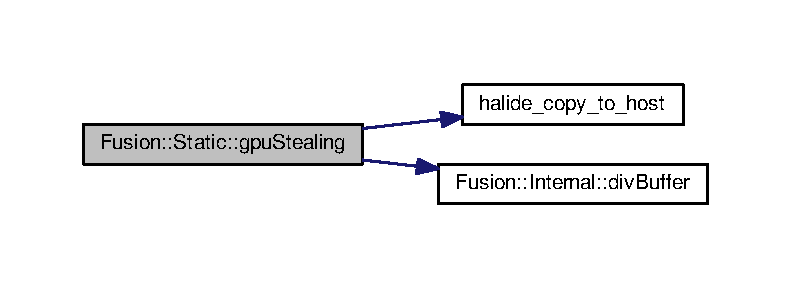
\includegraphics[width=350pt]{namespace_fusion_1_1_static_a4dda28311f1977091df5d7adb5aec742_cgraph}
\end{center}
\end{figure}


\hypertarget{namespace_fusion_1_1_static_a36302361627ccb126b6aeb0efa6d3ab2}{\index{Fusion\-::\-Static@{Fusion\-::\-Static}!gpu\-Thread@{gpu\-Thread}}
\index{gpu\-Thread@{gpu\-Thread}!Fusion::Static@{Fusion\-::\-Static}}
\subsubsection[{gpu\-Thread}]{\setlength{\rightskip}{0pt plus 5cm}template$<$typename... Args$>$ void Fusion\-::\-Static\-::gpu\-Thread (
\begin{DoxyParamCaption}
\item[{Args...}]{args, }
\item[{function$<$ int(Args..., {\bf buffer\-\_\-t} $\ast$, {\bf buffer\-\_\-t} $\ast$)$>$}]{func, }
\item[{{\bf buffer\-\_\-t} $\ast$}]{input, }
\item[{{\bf buffer\-\_\-t} $\ast$}]{output}
\end{DoxyParamCaption}
)}}\label{namespace_fusion_1_1_static_a36302361627ccb126b6aeb0efa6d3ab2}
This Function is a thread for \hyperlink{namespace_fusion_1_1_static}{Static} execution way W\-I\-T\-H\-O\-U\-T stealing. 

Here is the call graph for this function\-:
\nopagebreak
\begin{figure}[H]
\begin{center}
\leavevmode
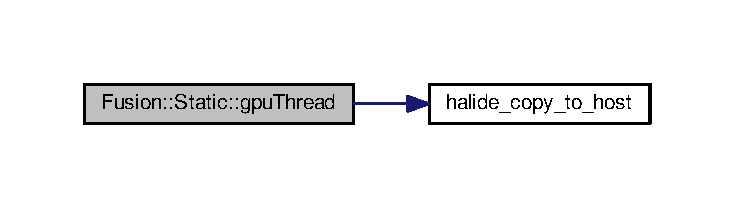
\includegraphics[width=350pt]{namespace_fusion_1_1_static_a36302361627ccb126b6aeb0efa6d3ab2_cgraph}
\end{center}
\end{figure}



\chapter{Class Documentation}
\hypertarget{structbuffer__t}{\section{buffer\-\_\-t Struct Reference}
\label{structbuffer__t}\index{buffer\-\_\-t@{buffer\-\_\-t}}
}


{\ttfamily \#include $<$fusion.\-h$>$}

\subsection*{Public Attributes}
\begin{DoxyCompactItemize}
\item 
uint64\-\_\-t \hyperlink{structbuffer__t_a6653bc34b20aa7c42bed9807d1111548}{dev}
\item 
uint8\-\_\-t $\ast$ \hyperlink{structbuffer__t_a48342b699f70a5399e892dfdfa271191}{host}
\item 
int32\-\_\-t \hyperlink{structbuffer__t_a8760bb291bb79576c6db5621edd2b4aa}{extent} \mbox{[}4\mbox{]}
\item 
int32\-\_\-t \hyperlink{structbuffer__t_a20a8d2dc77012a89ddfc2647ea15cb44}{stride} \mbox{[}4\mbox{]}
\item 
int32\-\_\-t \hyperlink{structbuffer__t_a1932b10069a734ee12e242b5b929e28a}{min} \mbox{[}4\mbox{]}
\item 
int32\-\_\-t \hyperlink{structbuffer__t_ae161a929ed7ed53425204ddcaf499c63}{elem\-\_\-size}
\item 
bool \hyperlink{structbuffer__t_a73a357ef44b1417a60ec0da43e9e0868}{host\-\_\-dirty}
\item 
bool \hyperlink{structbuffer__t_a6f8e9141729081246d3bfd1e6d1b376a}{dev\-\_\-dirty}
\end{DoxyCompactItemize}


\subsection{Member Data Documentation}
\hypertarget{structbuffer__t_a6653bc34b20aa7c42bed9807d1111548}{\index{buffer\-\_\-t@{buffer\-\_\-t}!dev@{dev}}
\index{dev@{dev}!buffer_t@{buffer\-\_\-t}}
\subsubsection[{dev}]{\setlength{\rightskip}{0pt plus 5cm}uint64\-\_\-t buffer\-\_\-t\-::dev}}\label{structbuffer__t_a6653bc34b20aa7c42bed9807d1111548}
\hypertarget{structbuffer__t_a6f8e9141729081246d3bfd1e6d1b376a}{\index{buffer\-\_\-t@{buffer\-\_\-t}!dev\-\_\-dirty@{dev\-\_\-dirty}}
\index{dev\-\_\-dirty@{dev\-\_\-dirty}!buffer_t@{buffer\-\_\-t}}
\subsubsection[{dev\-\_\-dirty}]{\setlength{\rightskip}{0pt plus 5cm}bool buffer\-\_\-t\-::dev\-\_\-dirty}}\label{structbuffer__t_a6f8e9141729081246d3bfd1e6d1b376a}
\hypertarget{structbuffer__t_ae161a929ed7ed53425204ddcaf499c63}{\index{buffer\-\_\-t@{buffer\-\_\-t}!elem\-\_\-size@{elem\-\_\-size}}
\index{elem\-\_\-size@{elem\-\_\-size}!buffer_t@{buffer\-\_\-t}}
\subsubsection[{elem\-\_\-size}]{\setlength{\rightskip}{0pt plus 5cm}int32\-\_\-t buffer\-\_\-t\-::elem\-\_\-size}}\label{structbuffer__t_ae161a929ed7ed53425204ddcaf499c63}
\hypertarget{structbuffer__t_a8760bb291bb79576c6db5621edd2b4aa}{\index{buffer\-\_\-t@{buffer\-\_\-t}!extent@{extent}}
\index{extent@{extent}!buffer_t@{buffer\-\_\-t}}
\subsubsection[{extent}]{\setlength{\rightskip}{0pt plus 5cm}int32\-\_\-t buffer\-\_\-t\-::extent}}\label{structbuffer__t_a8760bb291bb79576c6db5621edd2b4aa}
\hypertarget{structbuffer__t_a48342b699f70a5399e892dfdfa271191}{\index{buffer\-\_\-t@{buffer\-\_\-t}!host@{host}}
\index{host@{host}!buffer_t@{buffer\-\_\-t}}
\subsubsection[{host}]{\setlength{\rightskip}{0pt plus 5cm}uint8\-\_\-t $\ast$ buffer\-\_\-t\-::host}}\label{structbuffer__t_a48342b699f70a5399e892dfdfa271191}
\hypertarget{structbuffer__t_a73a357ef44b1417a60ec0da43e9e0868}{\index{buffer\-\_\-t@{buffer\-\_\-t}!host\-\_\-dirty@{host\-\_\-dirty}}
\index{host\-\_\-dirty@{host\-\_\-dirty}!buffer_t@{buffer\-\_\-t}}
\subsubsection[{host\-\_\-dirty}]{\setlength{\rightskip}{0pt plus 5cm}bool buffer\-\_\-t\-::host\-\_\-dirty}}\label{structbuffer__t_a73a357ef44b1417a60ec0da43e9e0868}
\hypertarget{structbuffer__t_a1932b10069a734ee12e242b5b929e28a}{\index{buffer\-\_\-t@{buffer\-\_\-t}!min@{min}}
\index{min@{min}!buffer_t@{buffer\-\_\-t}}
\subsubsection[{min}]{\setlength{\rightskip}{0pt plus 5cm}int32\-\_\-t buffer\-\_\-t\-::min}}\label{structbuffer__t_a1932b10069a734ee12e242b5b929e28a}
\hypertarget{structbuffer__t_a20a8d2dc77012a89ddfc2647ea15cb44}{\index{buffer\-\_\-t@{buffer\-\_\-t}!stride@{stride}}
\index{stride@{stride}!buffer_t@{buffer\-\_\-t}}
\subsubsection[{stride}]{\setlength{\rightskip}{0pt plus 5cm}int32\-\_\-t buffer\-\_\-t\-::stride}}\label{structbuffer__t_a20a8d2dc77012a89ddfc2647ea15cb44}


The documentation for this struct was generated from the following files\-:\begin{DoxyCompactItemize}
\item 
\hyperlink{fusion_8h}{fusion.\-h}\item 
\hyperlink{internal_8h}{internal.\-h}\end{DoxyCompactItemize}

\hypertarget{class_fusion_1_1_dynamic_1_1_dynamic_dispatch}{\section{Fusion\-:\-:Dynamic\-:\-:Dynamic\-Dispatch$<$ Args $>$ Class Template Reference}
\label{class_fusion_1_1_dynamic_1_1_dynamic_dispatch}\index{Fusion\-::\-Dynamic\-::\-Dynamic\-Dispatch$<$ Args $>$@{Fusion\-::\-Dynamic\-::\-Dynamic\-Dispatch$<$ Args $>$}}
}


{\ttfamily \#include $<$Dynamic\-Dispatch.\-h$>$}

\subsection*{Public Member Functions}
\begin{DoxyCompactItemize}
\item 
\hyperlink{class_fusion_1_1_dynamic_1_1_dynamic_dispatch_ad7f22c9e07d69a934a9f0c0adc1e256c}{Dynamic\-Dispatch} ()
\item 
\hyperlink{class_fusion_1_1_dynamic_1_1_dynamic_dispatch_a76a96462319d863ab9cc138f341cb43b}{Dynamic\-Dispatch} (function$<$ int(Args..., \hyperlink{structbuffer__t}{buffer\-\_\-t} $\ast$, \hyperlink{structbuffer__t}{buffer\-\_\-t} $\ast$)$>$ \-\_\-cpu\-Func, function$<$ int(Args..., \hyperlink{structbuffer__t}{buffer\-\_\-t} $\ast$, \hyperlink{structbuffer__t}{buffer\-\_\-t} $\ast$)$>$ \-\_\-gpu\-Func)
\item 
\hyperlink{class_fusion_1_1_dynamic_1_1_dynamic_dispatch_ad8465d30baed11928f7ec89aa7059622}{Dynamic\-Dispatch} (function$<$ int(Args..., \hyperlink{structbuffer__t}{buffer\-\_\-t} $\ast$, \hyperlink{structbuffer__t}{buffer\-\_\-t} $\ast$)$>$ \-\_\-cpu\-Func, function$<$ int(Args..., \hyperlink{structbuffer__t}{buffer\-\_\-t} $\ast$, \hyperlink{structbuffer__t}{buffer\-\_\-t} $\ast$)$>$ \-\_\-gpu\-Func, \hyperlink{structbuffer__t}{buffer\-\_\-t} $\ast$\-\_\-input)
\item 
\hyperlink{class_fusion_1_1_dynamic_1_1_dynamic_dispatch_aa13c90fe52064be5caa254f86a56d93f}{Dynamic\-Dispatch} (function$<$ int(Args..., \hyperlink{structbuffer__t}{buffer\-\_\-t} $\ast$, \hyperlink{structbuffer__t}{buffer\-\_\-t} $\ast$)$>$ \-\_\-cpu\-Func, function$<$ int(Args..., \hyperlink{structbuffer__t}{buffer\-\_\-t} $\ast$, \hyperlink{structbuffer__t}{buffer\-\_\-t} $\ast$)$>$ \-\_\-gpu\-Func, \hyperlink{structbuffer__t}{buffer\-\_\-t} $\ast$\-\_\-input, \hyperlink{structbuffer__t}{buffer\-\_\-t} $\ast$\-\_\-output)
\item 
int \hyperlink{class_fusion_1_1_dynamic_1_1_dynamic_dispatch_a9fafe72f2e1425c47f18bb3bab8601c4}{Realize} (Args...)
\item 
int \hyperlink{class_fusion_1_1_dynamic_1_1_dynamic_dispatch_a3e5d0db1df8ecf2376ef1a7073b3317f}{realize\-C\-P\-U} (Args...)
\item 
int \hyperlink{class_fusion_1_1_dynamic_1_1_dynamic_dispatch_a119f0f612ef66b521cb46dcdb2011b7a}{realize\-G\-P\-U} (Args...)
\item 
int \hyperlink{class_fusion_1_1_dynamic_1_1_dynamic_dispatch_a6a77f16d2d94f24a258619329b836495}{realize\-C\-P\-U} (Args..., \hyperlink{structbuffer__t}{buffer\-\_\-t} $\ast$\-\_\-output)
\item 
int \hyperlink{class_fusion_1_1_dynamic_1_1_dynamic_dispatch_adb32715cd6ad3be6db87589056a42e59}{realize\-G\-P\-U} (Args..., \hyperlink{structbuffer__t}{buffer\-\_\-t} $\ast$\-\_\-output)
\item 
void \hyperlink{class_fusion_1_1_dynamic_1_1_dynamic_dispatch_aa7a9f3d9a3a59ca49d4526dabfba3cbf}{set\-Input} (\hyperlink{structbuffer__t}{buffer\-\_\-t} $\ast$\-\_\-input)
\item 
void \hyperlink{class_fusion_1_1_dynamic_1_1_dynamic_dispatch_a8f26bf074900b28f551e5a2c9cd0ff1a}{set\-Output} (\hyperlink{structbuffer__t}{buffer\-\_\-t} $\ast$\-\_\-output)
\end{DoxyCompactItemize}
\subsection*{Public Attributes}
\begin{DoxyCompactItemize}
\item 
mutex $\ast$ \hyperlink{class_fusion_1_1_dynamic_1_1_dynamic_dispatch_a8416a4564562c331d2d9191526706302}{table\-\_\-mutex}
\end{DoxyCompactItemize}


\subsection{Constructor \& Destructor Documentation}
\hypertarget{class_fusion_1_1_dynamic_1_1_dynamic_dispatch_ad7f22c9e07d69a934a9f0c0adc1e256c}{\index{Fusion\-::\-Dynamic\-::\-Dynamic\-Dispatch@{Fusion\-::\-Dynamic\-::\-Dynamic\-Dispatch}!Dynamic\-Dispatch@{Dynamic\-Dispatch}}
\index{Dynamic\-Dispatch@{Dynamic\-Dispatch}!Fusion::Dynamic::DynamicDispatch@{Fusion\-::\-Dynamic\-::\-Dynamic\-Dispatch}}
\subsubsection[{Dynamic\-Dispatch}]{\setlength{\rightskip}{0pt plus 5cm}template$<$typename... Args$>$ {\bf Fusion\-::\-Dynamic\-::\-Dynamic\-Dispatch}$<$ Args $>$\-::{\bf Dynamic\-Dispatch} (
\begin{DoxyParamCaption}
{}
\end{DoxyParamCaption}
)\hspace{0.3cm}{\ttfamily [inline]}}}\label{class_fusion_1_1_dynamic_1_1_dynamic_dispatch_ad7f22c9e07d69a934a9f0c0adc1e256c}
\hypertarget{class_fusion_1_1_dynamic_1_1_dynamic_dispatch_a76a96462319d863ab9cc138f341cb43b}{\index{Fusion\-::\-Dynamic\-::\-Dynamic\-Dispatch@{Fusion\-::\-Dynamic\-::\-Dynamic\-Dispatch}!Dynamic\-Dispatch@{Dynamic\-Dispatch}}
\index{Dynamic\-Dispatch@{Dynamic\-Dispatch}!Fusion::Dynamic::DynamicDispatch@{Fusion\-::\-Dynamic\-::\-Dynamic\-Dispatch}}
\subsubsection[{Dynamic\-Dispatch}]{\setlength{\rightskip}{0pt plus 5cm}template$<$typename... Args$>$ {\bf Fusion\-::\-Dynamic\-::\-Dynamic\-Dispatch}$<$ Args $>$\-::{\bf Dynamic\-Dispatch} (
\begin{DoxyParamCaption}
\item[{function$<$ int(Args..., {\bf buffer\-\_\-t} $\ast$, {\bf buffer\-\_\-t} $\ast$)$>$}]{\-\_\-cpu\-Func, }
\item[{function$<$ int(Args..., {\bf buffer\-\_\-t} $\ast$, {\bf buffer\-\_\-t} $\ast$)$>$}]{\-\_\-gpu\-Func}
\end{DoxyParamCaption}
)\hspace{0.3cm}{\ttfamily [inline]}}}\label{class_fusion_1_1_dynamic_1_1_dynamic_dispatch_a76a96462319d863ab9cc138f341cb43b}
\hypertarget{class_fusion_1_1_dynamic_1_1_dynamic_dispatch_ad8465d30baed11928f7ec89aa7059622}{\index{Fusion\-::\-Dynamic\-::\-Dynamic\-Dispatch@{Fusion\-::\-Dynamic\-::\-Dynamic\-Dispatch}!Dynamic\-Dispatch@{Dynamic\-Dispatch}}
\index{Dynamic\-Dispatch@{Dynamic\-Dispatch}!Fusion::Dynamic::DynamicDispatch@{Fusion\-::\-Dynamic\-::\-Dynamic\-Dispatch}}
\subsubsection[{Dynamic\-Dispatch}]{\setlength{\rightskip}{0pt plus 5cm}template$<$typename... Args$>$ {\bf Fusion\-::\-Dynamic\-::\-Dynamic\-Dispatch}$<$ Args $>$\-::{\bf Dynamic\-Dispatch} (
\begin{DoxyParamCaption}
\item[{function$<$ int(Args..., {\bf buffer\-\_\-t} $\ast$, {\bf buffer\-\_\-t} $\ast$)$>$}]{\-\_\-cpu\-Func, }
\item[{function$<$ int(Args..., {\bf buffer\-\_\-t} $\ast$, {\bf buffer\-\_\-t} $\ast$)$>$}]{\-\_\-gpu\-Func, }
\item[{{\bf buffer\-\_\-t} $\ast$}]{\-\_\-input}
\end{DoxyParamCaption}
)\hspace{0.3cm}{\ttfamily [inline]}}}\label{class_fusion_1_1_dynamic_1_1_dynamic_dispatch_ad8465d30baed11928f7ec89aa7059622}
\hypertarget{class_fusion_1_1_dynamic_1_1_dynamic_dispatch_aa13c90fe52064be5caa254f86a56d93f}{\index{Fusion\-::\-Dynamic\-::\-Dynamic\-Dispatch@{Fusion\-::\-Dynamic\-::\-Dynamic\-Dispatch}!Dynamic\-Dispatch@{Dynamic\-Dispatch}}
\index{Dynamic\-Dispatch@{Dynamic\-Dispatch}!Fusion::Dynamic::DynamicDispatch@{Fusion\-::\-Dynamic\-::\-Dynamic\-Dispatch}}
\subsubsection[{Dynamic\-Dispatch}]{\setlength{\rightskip}{0pt plus 5cm}template$<$typename... Args$>$ {\bf Fusion\-::\-Dynamic\-::\-Dynamic\-Dispatch}$<$ Args $>$\-::{\bf Dynamic\-Dispatch} (
\begin{DoxyParamCaption}
\item[{function$<$ int(Args..., {\bf buffer\-\_\-t} $\ast$, {\bf buffer\-\_\-t} $\ast$)$>$}]{\-\_\-cpu\-Func, }
\item[{function$<$ int(Args..., {\bf buffer\-\_\-t} $\ast$, {\bf buffer\-\_\-t} $\ast$)$>$}]{\-\_\-gpu\-Func, }
\item[{{\bf buffer\-\_\-t} $\ast$}]{\-\_\-input, }
\item[{{\bf buffer\-\_\-t} $\ast$}]{\-\_\-output}
\end{DoxyParamCaption}
)\hspace{0.3cm}{\ttfamily [inline]}}}\label{class_fusion_1_1_dynamic_1_1_dynamic_dispatch_aa13c90fe52064be5caa254f86a56d93f}


\subsection{Member Function Documentation}
\hypertarget{class_fusion_1_1_dynamic_1_1_dynamic_dispatch_a9fafe72f2e1425c47f18bb3bab8601c4}{\index{Fusion\-::\-Dynamic\-::\-Dynamic\-Dispatch@{Fusion\-::\-Dynamic\-::\-Dynamic\-Dispatch}!Realize@{Realize}}
\index{Realize@{Realize}!Fusion::Dynamic::DynamicDispatch@{Fusion\-::\-Dynamic\-::\-Dynamic\-Dispatch}}
\subsubsection[{Realize}]{\setlength{\rightskip}{0pt plus 5cm}template$<$typename... Args$>$ int {\bf Fusion\-::\-Dynamic\-::\-Dynamic\-Dispatch}$<$ Args $>$\-::Realize (
\begin{DoxyParamCaption}
\item[{Args...}]{args}
\end{DoxyParamCaption}
)}}\label{class_fusion_1_1_dynamic_1_1_dynamic_dispatch_a9fafe72f2e1425c47f18bb3bab8601c4}


Here is the call graph for this function\-:
\nopagebreak
\begin{figure}[H]
\begin{center}
\leavevmode
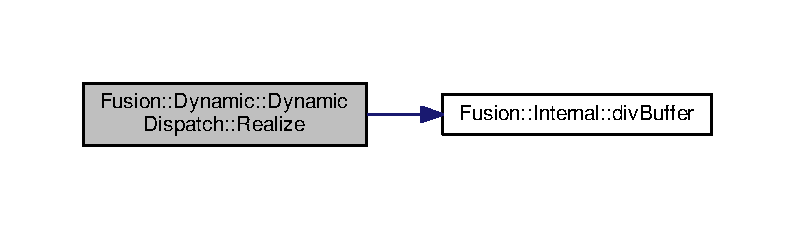
\includegraphics[width=350pt]{class_fusion_1_1_dynamic_1_1_dynamic_dispatch_a9fafe72f2e1425c47f18bb3bab8601c4_cgraph}
\end{center}
\end{figure}


\hypertarget{class_fusion_1_1_dynamic_1_1_dynamic_dispatch_a3e5d0db1df8ecf2376ef1a7073b3317f}{\index{Fusion\-::\-Dynamic\-::\-Dynamic\-Dispatch@{Fusion\-::\-Dynamic\-::\-Dynamic\-Dispatch}!realize\-C\-P\-U@{realize\-C\-P\-U}}
\index{realize\-C\-P\-U@{realize\-C\-P\-U}!Fusion::Dynamic::DynamicDispatch@{Fusion\-::\-Dynamic\-::\-Dynamic\-Dispatch}}
\subsubsection[{realize\-C\-P\-U}]{\setlength{\rightskip}{0pt plus 5cm}template$<$typename... Args$>$ int {\bf Fusion\-::\-Dynamic\-::\-Dynamic\-Dispatch}$<$ Args $>$\-::realize\-C\-P\-U (
\begin{DoxyParamCaption}
\item[{Args...}]{args}
\end{DoxyParamCaption}
)}}\label{class_fusion_1_1_dynamic_1_1_dynamic_dispatch_a3e5d0db1df8ecf2376ef1a7073b3317f}
\hypertarget{class_fusion_1_1_dynamic_1_1_dynamic_dispatch_a6a77f16d2d94f24a258619329b836495}{\index{Fusion\-::\-Dynamic\-::\-Dynamic\-Dispatch@{Fusion\-::\-Dynamic\-::\-Dynamic\-Dispatch}!realize\-C\-P\-U@{realize\-C\-P\-U}}
\index{realize\-C\-P\-U@{realize\-C\-P\-U}!Fusion::Dynamic::DynamicDispatch@{Fusion\-::\-Dynamic\-::\-Dynamic\-Dispatch}}
\subsubsection[{realize\-C\-P\-U}]{\setlength{\rightskip}{0pt plus 5cm}template$<$typename... Args$>$ int {\bf Fusion\-::\-Dynamic\-::\-Dynamic\-Dispatch}$<$ Args $>$\-::realize\-C\-P\-U (
\begin{DoxyParamCaption}
\item[{Args...}]{args, }
\item[{{\bf buffer\-\_\-t} $\ast$}]{\-\_\-output}
\end{DoxyParamCaption}
)}}\label{class_fusion_1_1_dynamic_1_1_dynamic_dispatch_a6a77f16d2d94f24a258619329b836495}
\hypertarget{class_fusion_1_1_dynamic_1_1_dynamic_dispatch_a119f0f612ef66b521cb46dcdb2011b7a}{\index{Fusion\-::\-Dynamic\-::\-Dynamic\-Dispatch@{Fusion\-::\-Dynamic\-::\-Dynamic\-Dispatch}!realize\-G\-P\-U@{realize\-G\-P\-U}}
\index{realize\-G\-P\-U@{realize\-G\-P\-U}!Fusion::Dynamic::DynamicDispatch@{Fusion\-::\-Dynamic\-::\-Dynamic\-Dispatch}}
\subsubsection[{realize\-G\-P\-U}]{\setlength{\rightskip}{0pt plus 5cm}template$<$typename... Args$>$ int {\bf Fusion\-::\-Dynamic\-::\-Dynamic\-Dispatch}$<$ Args $>$\-::realize\-G\-P\-U (
\begin{DoxyParamCaption}
\item[{Args...}]{args}
\end{DoxyParamCaption}
)}}\label{class_fusion_1_1_dynamic_1_1_dynamic_dispatch_a119f0f612ef66b521cb46dcdb2011b7a}


Here is the call graph for this function\-:
\nopagebreak
\begin{figure}[H]
\begin{center}
\leavevmode
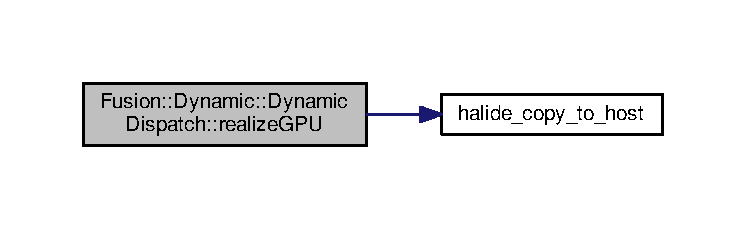
\includegraphics[width=350pt]{class_fusion_1_1_dynamic_1_1_dynamic_dispatch_a119f0f612ef66b521cb46dcdb2011b7a_cgraph}
\end{center}
\end{figure}


\hypertarget{class_fusion_1_1_dynamic_1_1_dynamic_dispatch_adb32715cd6ad3be6db87589056a42e59}{\index{Fusion\-::\-Dynamic\-::\-Dynamic\-Dispatch@{Fusion\-::\-Dynamic\-::\-Dynamic\-Dispatch}!realize\-G\-P\-U@{realize\-G\-P\-U}}
\index{realize\-G\-P\-U@{realize\-G\-P\-U}!Fusion::Dynamic::DynamicDispatch@{Fusion\-::\-Dynamic\-::\-Dynamic\-Dispatch}}
\subsubsection[{realize\-G\-P\-U}]{\setlength{\rightskip}{0pt plus 5cm}template$<$typename... Args$>$ int {\bf Fusion\-::\-Dynamic\-::\-Dynamic\-Dispatch}$<$ Args $>$\-::realize\-G\-P\-U (
\begin{DoxyParamCaption}
\item[{Args...}]{args, }
\item[{{\bf buffer\-\_\-t} $\ast$}]{\-\_\-output}
\end{DoxyParamCaption}
)}}\label{class_fusion_1_1_dynamic_1_1_dynamic_dispatch_adb32715cd6ad3be6db87589056a42e59}


Here is the call graph for this function\-:
\nopagebreak
\begin{figure}[H]
\begin{center}
\leavevmode
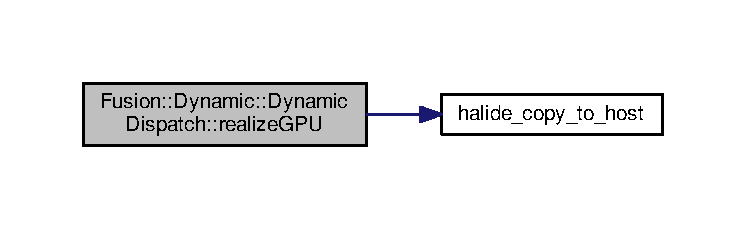
\includegraphics[width=350pt]{class_fusion_1_1_dynamic_1_1_dynamic_dispatch_adb32715cd6ad3be6db87589056a42e59_cgraph}
\end{center}
\end{figure}


\hypertarget{class_fusion_1_1_dynamic_1_1_dynamic_dispatch_aa7a9f3d9a3a59ca49d4526dabfba3cbf}{\index{Fusion\-::\-Dynamic\-::\-Dynamic\-Dispatch@{Fusion\-::\-Dynamic\-::\-Dynamic\-Dispatch}!set\-Input@{set\-Input}}
\index{set\-Input@{set\-Input}!Fusion::Dynamic::DynamicDispatch@{Fusion\-::\-Dynamic\-::\-Dynamic\-Dispatch}}
\subsubsection[{set\-Input}]{\setlength{\rightskip}{0pt plus 5cm}template$<$typename... Args$>$ void {\bf Fusion\-::\-Dynamic\-::\-Dynamic\-Dispatch}$<$ Args $>$\-::set\-Input (
\begin{DoxyParamCaption}
\item[{{\bf buffer\-\_\-t} $\ast$}]{\-\_\-input}
\end{DoxyParamCaption}
)\hspace{0.3cm}{\ttfamily [inline]}}}\label{class_fusion_1_1_dynamic_1_1_dynamic_dispatch_aa7a9f3d9a3a59ca49d4526dabfba3cbf}
\hypertarget{class_fusion_1_1_dynamic_1_1_dynamic_dispatch_a8f26bf074900b28f551e5a2c9cd0ff1a}{\index{Fusion\-::\-Dynamic\-::\-Dynamic\-Dispatch@{Fusion\-::\-Dynamic\-::\-Dynamic\-Dispatch}!set\-Output@{set\-Output}}
\index{set\-Output@{set\-Output}!Fusion::Dynamic::DynamicDispatch@{Fusion\-::\-Dynamic\-::\-Dynamic\-Dispatch}}
\subsubsection[{set\-Output}]{\setlength{\rightskip}{0pt plus 5cm}template$<$typename... Args$>$ void {\bf Fusion\-::\-Dynamic\-::\-Dynamic\-Dispatch}$<$ Args $>$\-::set\-Output (
\begin{DoxyParamCaption}
\item[{{\bf buffer\-\_\-t} $\ast$}]{\-\_\-output}
\end{DoxyParamCaption}
)\hspace{0.3cm}{\ttfamily [inline]}}}\label{class_fusion_1_1_dynamic_1_1_dynamic_dispatch_a8f26bf074900b28f551e5a2c9cd0ff1a}


\subsection{Member Data Documentation}
\hypertarget{class_fusion_1_1_dynamic_1_1_dynamic_dispatch_a8416a4564562c331d2d9191526706302}{\index{Fusion\-::\-Dynamic\-::\-Dynamic\-Dispatch@{Fusion\-::\-Dynamic\-::\-Dynamic\-Dispatch}!table\-\_\-mutex@{table\-\_\-mutex}}
\index{table\-\_\-mutex@{table\-\_\-mutex}!Fusion::Dynamic::DynamicDispatch@{Fusion\-::\-Dynamic\-::\-Dynamic\-Dispatch}}
\subsubsection[{table\-\_\-mutex}]{\setlength{\rightskip}{0pt plus 5cm}template$<$typename... Args$>$ mutex$\ast$ {\bf Fusion\-::\-Dynamic\-::\-Dynamic\-Dispatch}$<$ Args $>$\-::table\-\_\-mutex}}\label{class_fusion_1_1_dynamic_1_1_dynamic_dispatch_a8416a4564562c331d2d9191526706302}


The documentation for this class was generated from the following file\-:\begin{DoxyCompactItemize}
\item 
\hyperlink{_dynamic_dispatch_8h}{Dynamic\-Dispatch.\-h}\end{DoxyCompactItemize}

\hypertarget{class_fusion_1_1_static_1_1_static_dispatch}{\section{Fusion\-:\-:Static\-:\-:Static\-Dispatch$<$ Args $>$ Class Template Reference}
\label{class_fusion_1_1_static_1_1_static_dispatch}\index{Fusion\-::\-Static\-::\-Static\-Dispatch$<$ Args $>$@{Fusion\-::\-Static\-::\-Static\-Dispatch$<$ Args $>$}}
}


{\ttfamily \#include $<$Static\-Dispatch.\-h$>$}

\subsection*{Public Member Functions}
\begin{DoxyCompactItemize}
\item 
\hyperlink{class_fusion_1_1_static_1_1_static_dispatch_aec9bc8e9761fe734f393c2f45c38062c}{Static\-Dispatch} ()
\item 
\hyperlink{class_fusion_1_1_static_1_1_static_dispatch_a5cfebb05577106e1d07d643df71ffdae}{Static\-Dispatch} (function$<$ int(Args..., \hyperlink{structbuffer__t}{buffer\-\_\-t} $\ast$, \hyperlink{structbuffer__t}{buffer\-\_\-t} $\ast$)$>$ \-\_\-cpu\-Func, function$<$ int(Args..., \hyperlink{structbuffer__t}{buffer\-\_\-t} $\ast$, \hyperlink{structbuffer__t}{buffer\-\_\-t} $\ast$)$>$ \-\_\-gpu\-Func)
\item 
\hyperlink{class_fusion_1_1_static_1_1_static_dispatch_a3dd9cbf018bc5cb2bd79a18535c59247}{Static\-Dispatch} (function$<$ int(Args..., \hyperlink{structbuffer__t}{buffer\-\_\-t} $\ast$, \hyperlink{structbuffer__t}{buffer\-\_\-t} $\ast$)$>$ \-\_\-cpu\-Func, function$<$ int(Args..., \hyperlink{structbuffer__t}{buffer\-\_\-t} $\ast$, \hyperlink{structbuffer__t}{buffer\-\_\-t} $\ast$)$>$ \-\_\-gpu\-Func, \hyperlink{structbuffer__t}{buffer\-\_\-t} $\ast$\-\_\-input)
\item 
\hyperlink{class_fusion_1_1_static_1_1_static_dispatch_a2149402c6452471ae5652cace75b3de0}{Static\-Dispatch} (function$<$ int(Args..., \hyperlink{structbuffer__t}{buffer\-\_\-t} $\ast$, \hyperlink{structbuffer__t}{buffer\-\_\-t} $\ast$)$>$ \-\_\-cpu\-Func, function$<$ int(Args..., \hyperlink{structbuffer__t}{buffer\-\_\-t} $\ast$, \hyperlink{structbuffer__t}{buffer\-\_\-t} $\ast$)$>$ \-\_\-gpu\-Func, \hyperlink{structbuffer__t}{buffer\-\_\-t} $\ast$\-\_\-input, \hyperlink{structbuffer__t}{buffer\-\_\-t} $\ast$\-\_\-output)
\item 
int \hyperlink{class_fusion_1_1_static_1_1_static_dispatch_ac74fd593ecfdd0c17cd3efb057a23601}{realize\-C\-P\-U} (Args...)
\item 
int \hyperlink{class_fusion_1_1_static_1_1_static_dispatch_a58ebbf76aad64618f27a051393cf06ac}{realize\-G\-P\-U} (Args...)
\item 
int \hyperlink{class_fusion_1_1_static_1_1_static_dispatch_a5242c852017c8bff8e2758da82fdfcdc}{realize\-C\-P\-U} (Args..., \hyperlink{structbuffer__t}{buffer\-\_\-t} $\ast$\-\_\-output)
\item 
int \hyperlink{class_fusion_1_1_static_1_1_static_dispatch_aa49de8865a4152db390e546dd17690a5}{realize\-G\-P\-U} (Args..., \hyperlink{structbuffer__t}{buffer\-\_\-t} $\ast$\-\_\-output)
\item 
int \hyperlink{class_fusion_1_1_static_1_1_static_dispatch_ad778f6d90895d75b920b173e2331d193}{realize\-With\-Stealing} (Args...\-args, int s)
\item 
void \hyperlink{class_fusion_1_1_static_1_1_static_dispatch_ab82336c566e180be617f49c708cdf7f0}{set\-Input} (\hyperlink{structbuffer__t}{buffer\-\_\-t} $\ast$\-\_\-input)
\item 
void \hyperlink{class_fusion_1_1_static_1_1_static_dispatch_a7c3cb7fa73040dbe2cfcbc3038119e48}{set\-Output} (\hyperlink{structbuffer__t}{buffer\-\_\-t} $\ast$\-\_\-output)
\item 
int \hyperlink{class_fusion_1_1_static_1_1_static_dispatch_ae167b1f550c4cc5260834109de6e5797}{realize} (Args..., int s)
\item 
int \hyperlink{class_fusion_1_1_static_1_1_static_dispatch_a4756d0081a1b0211d8f977a7b3aae110}{realize} (Args..., int s, int kernal\-Size)
\end{DoxyCompactItemize}
\subsection*{Public Attributes}
\begin{DoxyCompactItemize}
\item 
mutex $\ast$ \hyperlink{class_fusion_1_1_static_1_1_static_dispatch_adcf07c56b063db9d5aaa8eed6107d4b5}{table\-\_\-mutex}
\end{DoxyCompactItemize}


\subsection{Constructor \& Destructor Documentation}
\hypertarget{class_fusion_1_1_static_1_1_static_dispatch_aec9bc8e9761fe734f393c2f45c38062c}{\index{Fusion\-::\-Static\-::\-Static\-Dispatch@{Fusion\-::\-Static\-::\-Static\-Dispatch}!Static\-Dispatch@{Static\-Dispatch}}
\index{Static\-Dispatch@{Static\-Dispatch}!Fusion::Static::StaticDispatch@{Fusion\-::\-Static\-::\-Static\-Dispatch}}
\subsubsection[{Static\-Dispatch}]{\setlength{\rightskip}{0pt plus 5cm}template$<$typename... Args$>$ {\bf Fusion\-::\-Static\-::\-Static\-Dispatch}$<$ Args $>$\-::{\bf Static\-Dispatch} (
\begin{DoxyParamCaption}
{}
\end{DoxyParamCaption}
)\hspace{0.3cm}{\ttfamily [inline]}}}\label{class_fusion_1_1_static_1_1_static_dispatch_aec9bc8e9761fe734f393c2f45c38062c}
\hypertarget{class_fusion_1_1_static_1_1_static_dispatch_a5cfebb05577106e1d07d643df71ffdae}{\index{Fusion\-::\-Static\-::\-Static\-Dispatch@{Fusion\-::\-Static\-::\-Static\-Dispatch}!Static\-Dispatch@{Static\-Dispatch}}
\index{Static\-Dispatch@{Static\-Dispatch}!Fusion::Static::StaticDispatch@{Fusion\-::\-Static\-::\-Static\-Dispatch}}
\subsubsection[{Static\-Dispatch}]{\setlength{\rightskip}{0pt plus 5cm}template$<$typename... Args$>$ {\bf Fusion\-::\-Static\-::\-Static\-Dispatch}$<$ Args $>$\-::{\bf Static\-Dispatch} (
\begin{DoxyParamCaption}
\item[{function$<$ int(Args..., {\bf buffer\-\_\-t} $\ast$, {\bf buffer\-\_\-t} $\ast$)$>$}]{\-\_\-cpu\-Func, }
\item[{function$<$ int(Args..., {\bf buffer\-\_\-t} $\ast$, {\bf buffer\-\_\-t} $\ast$)$>$}]{\-\_\-gpu\-Func}
\end{DoxyParamCaption}
)\hspace{0.3cm}{\ttfamily [inline]}}}\label{class_fusion_1_1_static_1_1_static_dispatch_a5cfebb05577106e1d07d643df71ffdae}
\hypertarget{class_fusion_1_1_static_1_1_static_dispatch_a3dd9cbf018bc5cb2bd79a18535c59247}{\index{Fusion\-::\-Static\-::\-Static\-Dispatch@{Fusion\-::\-Static\-::\-Static\-Dispatch}!Static\-Dispatch@{Static\-Dispatch}}
\index{Static\-Dispatch@{Static\-Dispatch}!Fusion::Static::StaticDispatch@{Fusion\-::\-Static\-::\-Static\-Dispatch}}
\subsubsection[{Static\-Dispatch}]{\setlength{\rightskip}{0pt plus 5cm}template$<$typename... Args$>$ {\bf Fusion\-::\-Static\-::\-Static\-Dispatch}$<$ Args $>$\-::{\bf Static\-Dispatch} (
\begin{DoxyParamCaption}
\item[{function$<$ int(Args..., {\bf buffer\-\_\-t} $\ast$, {\bf buffer\-\_\-t} $\ast$)$>$}]{\-\_\-cpu\-Func, }
\item[{function$<$ int(Args..., {\bf buffer\-\_\-t} $\ast$, {\bf buffer\-\_\-t} $\ast$)$>$}]{\-\_\-gpu\-Func, }
\item[{{\bf buffer\-\_\-t} $\ast$}]{\-\_\-input}
\end{DoxyParamCaption}
)\hspace{0.3cm}{\ttfamily [inline]}}}\label{class_fusion_1_1_static_1_1_static_dispatch_a3dd9cbf018bc5cb2bd79a18535c59247}
\hypertarget{class_fusion_1_1_static_1_1_static_dispatch_a2149402c6452471ae5652cace75b3de0}{\index{Fusion\-::\-Static\-::\-Static\-Dispatch@{Fusion\-::\-Static\-::\-Static\-Dispatch}!Static\-Dispatch@{Static\-Dispatch}}
\index{Static\-Dispatch@{Static\-Dispatch}!Fusion::Static::StaticDispatch@{Fusion\-::\-Static\-::\-Static\-Dispatch}}
\subsubsection[{Static\-Dispatch}]{\setlength{\rightskip}{0pt plus 5cm}template$<$typename... Args$>$ {\bf Fusion\-::\-Static\-::\-Static\-Dispatch}$<$ Args $>$\-::{\bf Static\-Dispatch} (
\begin{DoxyParamCaption}
\item[{function$<$ int(Args..., {\bf buffer\-\_\-t} $\ast$, {\bf buffer\-\_\-t} $\ast$)$>$}]{\-\_\-cpu\-Func, }
\item[{function$<$ int(Args..., {\bf buffer\-\_\-t} $\ast$, {\bf buffer\-\_\-t} $\ast$)$>$}]{\-\_\-gpu\-Func, }
\item[{{\bf buffer\-\_\-t} $\ast$}]{\-\_\-input, }
\item[{{\bf buffer\-\_\-t} $\ast$}]{\-\_\-output}
\end{DoxyParamCaption}
)\hspace{0.3cm}{\ttfamily [inline]}}}\label{class_fusion_1_1_static_1_1_static_dispatch_a2149402c6452471ae5652cace75b3de0}


\subsection{Member Function Documentation}
\hypertarget{class_fusion_1_1_static_1_1_static_dispatch_ae167b1f550c4cc5260834109de6e5797}{\index{Fusion\-::\-Static\-::\-Static\-Dispatch@{Fusion\-::\-Static\-::\-Static\-Dispatch}!realize@{realize}}
\index{realize@{realize}!Fusion::Static::StaticDispatch@{Fusion\-::\-Static\-::\-Static\-Dispatch}}
\subsubsection[{realize}]{\setlength{\rightskip}{0pt plus 5cm}template$<$typename... Args$>$ int {\bf Fusion\-::\-Static\-::\-Static\-Dispatch}$<$ Args $>$\-::realize (
\begin{DoxyParamCaption}
\item[{Args...}]{args, }
\item[{int}]{s}
\end{DoxyParamCaption}
)}}\label{class_fusion_1_1_static_1_1_static_dispatch_ae167b1f550c4cc5260834109de6e5797}


Here is the call graph for this function\-:
\nopagebreak
\begin{figure}[H]
\begin{center}
\leavevmode
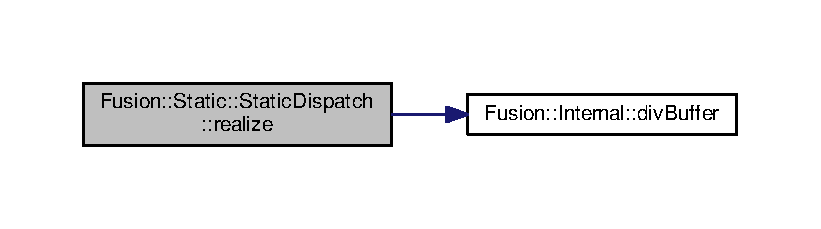
\includegraphics[width=350pt]{class_fusion_1_1_static_1_1_static_dispatch_ae167b1f550c4cc5260834109de6e5797_cgraph}
\end{center}
\end{figure}


\hypertarget{class_fusion_1_1_static_1_1_static_dispatch_a4756d0081a1b0211d8f977a7b3aae110}{\index{Fusion\-::\-Static\-::\-Static\-Dispatch@{Fusion\-::\-Static\-::\-Static\-Dispatch}!realize@{realize}}
\index{realize@{realize}!Fusion::Static::StaticDispatch@{Fusion\-::\-Static\-::\-Static\-Dispatch}}
\subsubsection[{realize}]{\setlength{\rightskip}{0pt plus 5cm}template$<$typename... Args$>$ int {\bf Fusion\-::\-Static\-::\-Static\-Dispatch}$<$ Args $>$\-::realize (
\begin{DoxyParamCaption}
\item[{Args...}]{args, }
\item[{int}]{s, }
\item[{int}]{kernal\-Size}
\end{DoxyParamCaption}
)}}\label{class_fusion_1_1_static_1_1_static_dispatch_a4756d0081a1b0211d8f977a7b3aae110}


Here is the call graph for this function\-:
\nopagebreak
\begin{figure}[H]
\begin{center}
\leavevmode
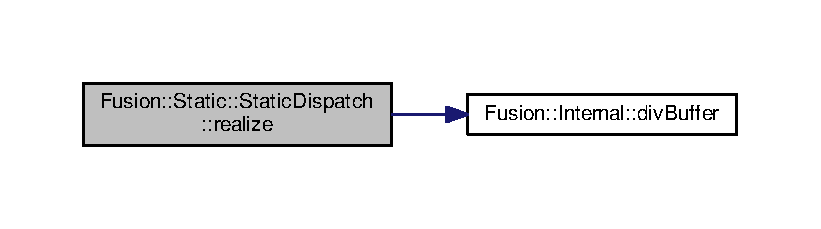
\includegraphics[width=350pt]{class_fusion_1_1_static_1_1_static_dispatch_a4756d0081a1b0211d8f977a7b3aae110_cgraph}
\end{center}
\end{figure}


\hypertarget{class_fusion_1_1_static_1_1_static_dispatch_ac74fd593ecfdd0c17cd3efb057a23601}{\index{Fusion\-::\-Static\-::\-Static\-Dispatch@{Fusion\-::\-Static\-::\-Static\-Dispatch}!realize\-C\-P\-U@{realize\-C\-P\-U}}
\index{realize\-C\-P\-U@{realize\-C\-P\-U}!Fusion::Static::StaticDispatch@{Fusion\-::\-Static\-::\-Static\-Dispatch}}
\subsubsection[{realize\-C\-P\-U}]{\setlength{\rightskip}{0pt plus 5cm}template$<$typename... Args$>$ int {\bf Fusion\-::\-Static\-::\-Static\-Dispatch}$<$ Args $>$\-::realize\-C\-P\-U (
\begin{DoxyParamCaption}
\item[{Args...}]{args}
\end{DoxyParamCaption}
)}}\label{class_fusion_1_1_static_1_1_static_dispatch_ac74fd593ecfdd0c17cd3efb057a23601}
For using C\-P\-U only \hypertarget{class_fusion_1_1_static_1_1_static_dispatch_a5242c852017c8bff8e2758da82fdfcdc}{\index{Fusion\-::\-Static\-::\-Static\-Dispatch@{Fusion\-::\-Static\-::\-Static\-Dispatch}!realize\-C\-P\-U@{realize\-C\-P\-U}}
\index{realize\-C\-P\-U@{realize\-C\-P\-U}!Fusion::Static::StaticDispatch@{Fusion\-::\-Static\-::\-Static\-Dispatch}}
\subsubsection[{realize\-C\-P\-U}]{\setlength{\rightskip}{0pt plus 5cm}template$<$typename... Args$>$ int {\bf Fusion\-::\-Static\-::\-Static\-Dispatch}$<$ Args $>$\-::realize\-C\-P\-U (
\begin{DoxyParamCaption}
\item[{Args...}]{args, }
\item[{{\bf buffer\-\_\-t} $\ast$}]{\-\_\-output}
\end{DoxyParamCaption}
)}}\label{class_fusion_1_1_static_1_1_static_dispatch_a5242c852017c8bff8e2758da82fdfcdc}
\hypertarget{class_fusion_1_1_static_1_1_static_dispatch_a58ebbf76aad64618f27a051393cf06ac}{\index{Fusion\-::\-Static\-::\-Static\-Dispatch@{Fusion\-::\-Static\-::\-Static\-Dispatch}!realize\-G\-P\-U@{realize\-G\-P\-U}}
\index{realize\-G\-P\-U@{realize\-G\-P\-U}!Fusion::Static::StaticDispatch@{Fusion\-::\-Static\-::\-Static\-Dispatch}}
\subsubsection[{realize\-G\-P\-U}]{\setlength{\rightskip}{0pt plus 5cm}template$<$typename... Args$>$ int {\bf Fusion\-::\-Static\-::\-Static\-Dispatch}$<$ Args $>$\-::realize\-G\-P\-U (
\begin{DoxyParamCaption}
\item[{Args...}]{args}
\end{DoxyParamCaption}
)}}\label{class_fusion_1_1_static_1_1_static_dispatch_a58ebbf76aad64618f27a051393cf06ac}


Here is the call graph for this function\-:
\nopagebreak
\begin{figure}[H]
\begin{center}
\leavevmode
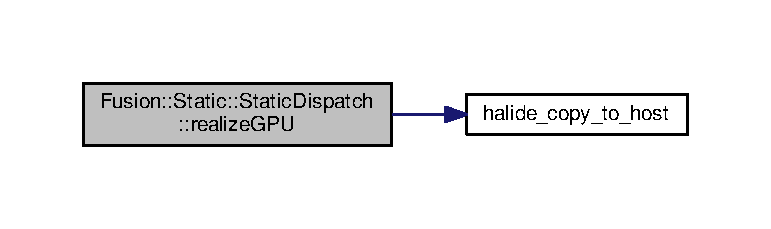
\includegraphics[width=350pt]{class_fusion_1_1_static_1_1_static_dispatch_a58ebbf76aad64618f27a051393cf06ac_cgraph}
\end{center}
\end{figure}


\hypertarget{class_fusion_1_1_static_1_1_static_dispatch_aa49de8865a4152db390e546dd17690a5}{\index{Fusion\-::\-Static\-::\-Static\-Dispatch@{Fusion\-::\-Static\-::\-Static\-Dispatch}!realize\-G\-P\-U@{realize\-G\-P\-U}}
\index{realize\-G\-P\-U@{realize\-G\-P\-U}!Fusion::Static::StaticDispatch@{Fusion\-::\-Static\-::\-Static\-Dispatch}}
\subsubsection[{realize\-G\-P\-U}]{\setlength{\rightskip}{0pt plus 5cm}template$<$typename... Args$>$ int {\bf Fusion\-::\-Static\-::\-Static\-Dispatch}$<$ Args $>$\-::realize\-G\-P\-U (
\begin{DoxyParamCaption}
\item[{Args...}]{args, }
\item[{{\bf buffer\-\_\-t} $\ast$}]{\-\_\-output}
\end{DoxyParamCaption}
)}}\label{class_fusion_1_1_static_1_1_static_dispatch_aa49de8865a4152db390e546dd17690a5}


Here is the call graph for this function\-:
\nopagebreak
\begin{figure}[H]
\begin{center}
\leavevmode
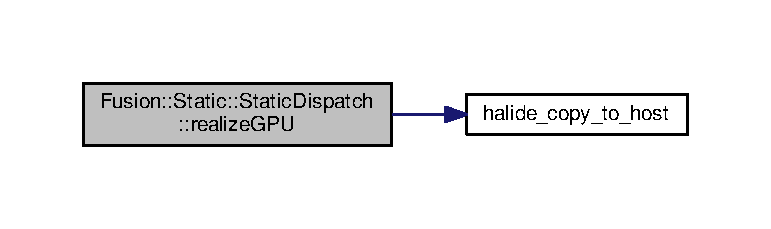
\includegraphics[width=350pt]{class_fusion_1_1_static_1_1_static_dispatch_aa49de8865a4152db390e546dd17690a5_cgraph}
\end{center}
\end{figure}


\hypertarget{class_fusion_1_1_static_1_1_static_dispatch_ad778f6d90895d75b920b173e2331d193}{\index{Fusion\-::\-Static\-::\-Static\-Dispatch@{Fusion\-::\-Static\-::\-Static\-Dispatch}!realize\-With\-Stealing@{realize\-With\-Stealing}}
\index{realize\-With\-Stealing@{realize\-With\-Stealing}!Fusion::Static::StaticDispatch@{Fusion\-::\-Static\-::\-Static\-Dispatch}}
\subsubsection[{realize\-With\-Stealing}]{\setlength{\rightskip}{0pt plus 5cm}template$<$typename... Args$>$ int {\bf Fusion\-::\-Static\-::\-Static\-Dispatch}$<$ Args $>$\-::realize\-With\-Stealing (
\begin{DoxyParamCaption}
\item[{Args...}]{args, }
\item[{int}]{s}
\end{DoxyParamCaption}
)}}\label{class_fusion_1_1_static_1_1_static_dispatch_ad778f6d90895d75b920b173e2331d193}


Here is the call graph for this function\-:
\nopagebreak
\begin{figure}[H]
\begin{center}
\leavevmode
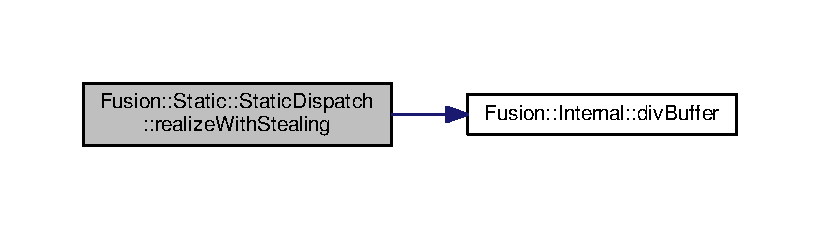
\includegraphics[width=350pt]{class_fusion_1_1_static_1_1_static_dispatch_ad778f6d90895d75b920b173e2331d193_cgraph}
\end{center}
\end{figure}


\hypertarget{class_fusion_1_1_static_1_1_static_dispatch_ab82336c566e180be617f49c708cdf7f0}{\index{Fusion\-::\-Static\-::\-Static\-Dispatch@{Fusion\-::\-Static\-::\-Static\-Dispatch}!set\-Input@{set\-Input}}
\index{set\-Input@{set\-Input}!Fusion::Static::StaticDispatch@{Fusion\-::\-Static\-::\-Static\-Dispatch}}
\subsubsection[{set\-Input}]{\setlength{\rightskip}{0pt plus 5cm}template$<$typename... Args$>$ void {\bf Fusion\-::\-Static\-::\-Static\-Dispatch}$<$ Args $>$\-::set\-Input (
\begin{DoxyParamCaption}
\item[{{\bf buffer\-\_\-t} $\ast$}]{\-\_\-input}
\end{DoxyParamCaption}
)\hspace{0.3cm}{\ttfamily [inline]}}}\label{class_fusion_1_1_static_1_1_static_dispatch_ab82336c566e180be617f49c708cdf7f0}
\hypertarget{class_fusion_1_1_static_1_1_static_dispatch_a7c3cb7fa73040dbe2cfcbc3038119e48}{\index{Fusion\-::\-Static\-::\-Static\-Dispatch@{Fusion\-::\-Static\-::\-Static\-Dispatch}!set\-Output@{set\-Output}}
\index{set\-Output@{set\-Output}!Fusion::Static::StaticDispatch@{Fusion\-::\-Static\-::\-Static\-Dispatch}}
\subsubsection[{set\-Output}]{\setlength{\rightskip}{0pt plus 5cm}template$<$typename... Args$>$ void {\bf Fusion\-::\-Static\-::\-Static\-Dispatch}$<$ Args $>$\-::set\-Output (
\begin{DoxyParamCaption}
\item[{{\bf buffer\-\_\-t} $\ast$}]{\-\_\-output}
\end{DoxyParamCaption}
)\hspace{0.3cm}{\ttfamily [inline]}}}\label{class_fusion_1_1_static_1_1_static_dispatch_a7c3cb7fa73040dbe2cfcbc3038119e48}


\subsection{Member Data Documentation}
\hypertarget{class_fusion_1_1_static_1_1_static_dispatch_adcf07c56b063db9d5aaa8eed6107d4b5}{\index{Fusion\-::\-Static\-::\-Static\-Dispatch@{Fusion\-::\-Static\-::\-Static\-Dispatch}!table\-\_\-mutex@{table\-\_\-mutex}}
\index{table\-\_\-mutex@{table\-\_\-mutex}!Fusion::Static::StaticDispatch@{Fusion\-::\-Static\-::\-Static\-Dispatch}}
\subsubsection[{table\-\_\-mutex}]{\setlength{\rightskip}{0pt plus 5cm}template$<$typename... Args$>$ mutex$\ast$ {\bf Fusion\-::\-Static\-::\-Static\-Dispatch}$<$ Args $>$\-::table\-\_\-mutex}}\label{class_fusion_1_1_static_1_1_static_dispatch_adcf07c56b063db9d5aaa8eed6107d4b5}


The documentation for this class was generated from the following file\-:\begin{DoxyCompactItemize}
\item 
\hyperlink{_static_dispatch_8h}{Static\-Dispatch.\-h}\end{DoxyCompactItemize}

\chapter{File Documentation}
\hypertarget{_dynamic_dispatch_8h}{\section{Dynamic\-Dispatch.\-h File Reference}
\label{_dynamic_dispatch_8h}\index{Dynamic\-Dispatch.\-h@{Dynamic\-Dispatch.\-h}}
}
{\ttfamily \#include \char`\"{}fusion.\-h\char`\"{}}\\*
Include dependency graph for Dynamic\-Dispatch.\-h\-:
\nopagebreak
\begin{figure}[H]
\begin{center}
\leavevmode
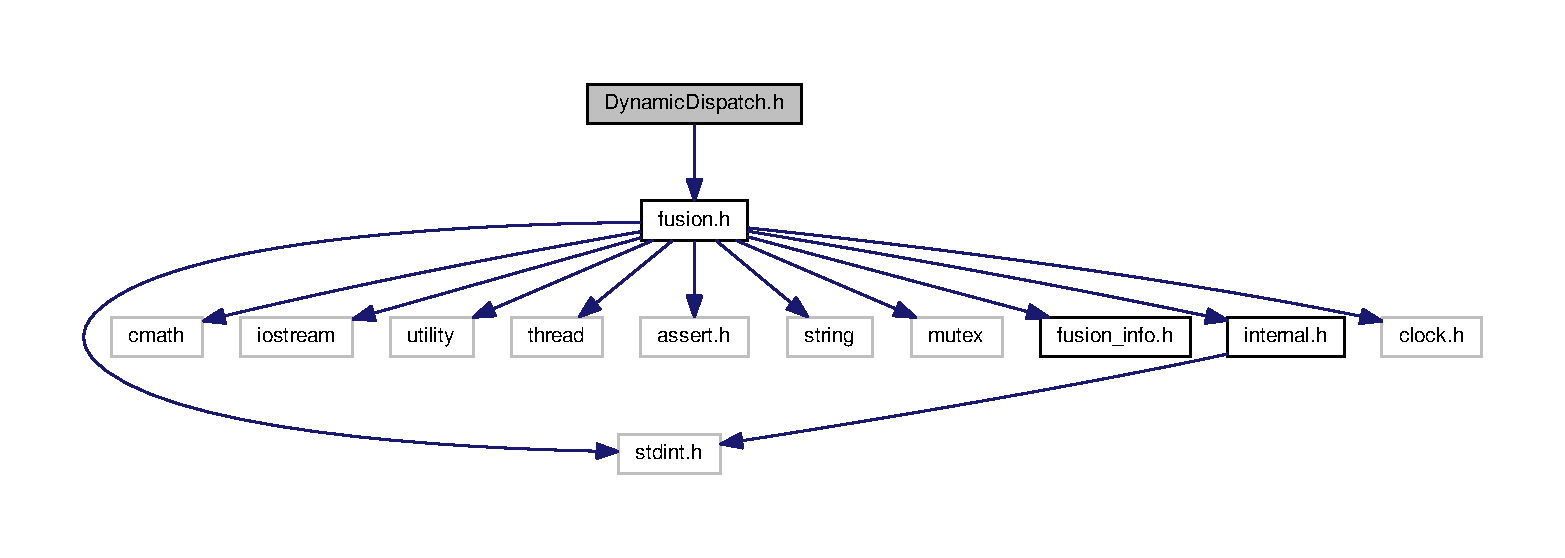
\includegraphics[width=350pt]{_dynamic_dispatch_8h__incl}
\end{center}
\end{figure}
\subsection*{Classes}
\begin{DoxyCompactItemize}
\item 
class \hyperlink{class_fusion_1_1_dynamic_1_1_dynamic_dispatch}{Fusion\-::\-Dynamic\-::\-Dynamic\-Dispatch$<$ Args $>$}
\end{DoxyCompactItemize}
\subsection*{Namespaces}
\begin{DoxyCompactItemize}
\item 
\hyperlink{namespace_fusion}{Fusion}
\item 
\hyperlink{namespace_fusion_1_1_dynamic}{Fusion\-::\-Dynamic}
\end{DoxyCompactItemize}
\subsection*{Functions}
\begin{DoxyCompactItemize}
\item 
{\footnotesize template$<$typename... Args$>$ }\\void \hyperlink{namespace_fusion_1_1_dynamic_a152d31c37efe7c83af9d8f899fe80f3e}{Fusion\-::\-Dynamic\-::work\-Thread} (Args...\-args, function$<$ int(Args..., \hyperlink{structbuffer__t}{buffer\-\_\-t} $\ast$, \hyperlink{structbuffer__t}{buffer\-\_\-t} $\ast$)$>$ func, \hyperlink{structbuffer__t}{buffer\-\_\-t} $\ast$input, \hyperlink{structbuffer__t}{buffer\-\_\-t} $\ast$output, \hyperlink{fusion__info_8h_a015eb90e0de9f16e87bd149d4b9ce959}{status} table\mbox{[}$\,$\mbox{]}, int offset, mutex $\ast$table\-\_\-mutex)
\end{DoxyCompactItemize}

\hypertarget{fusion_8h}{\section{fusion.\-h File Reference}
\label{fusion_8h}\index{fusion.\-h@{fusion.\-h}}
}
{\ttfamily \#include $<$stdint.\-h$>$}\\*
{\ttfamily \#include $<$cmath$>$}\\*
{\ttfamily \#include $<$iostream$>$}\\*
{\ttfamily \#include $<$utility$>$}\\*
{\ttfamily \#include $<$thread$>$}\\*
{\ttfamily \#include $<$assert.\-h$>$}\\*
{\ttfamily \#include $<$string$>$}\\*
{\ttfamily \#include $<$mutex$>$}\\*
{\ttfamily \#include \char`\"{}fusion\-\_\-info.\-h\char`\"{}}\\*
{\ttfamily \#include \char`\"{}internal.\-h\char`\"{}}\\*
{\ttfamily \#include \char`\"{}clock.\-h\char`\"{}}\\*
Include dependency graph for fusion.\-h\-:
\nopagebreak
\begin{figure}[H]
\begin{center}
\leavevmode
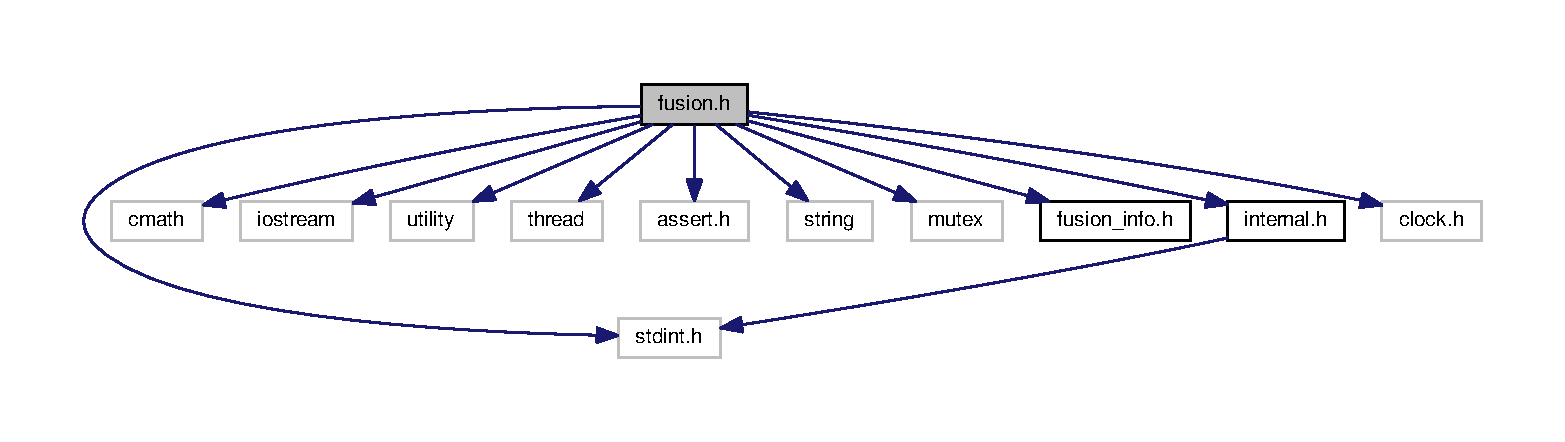
\includegraphics[width=350pt]{fusion_8h__incl}
\end{center}
\end{figure}
This graph shows which files directly or indirectly include this file\-:
\nopagebreak
\begin{figure}[H]
\begin{center}
\leavevmode
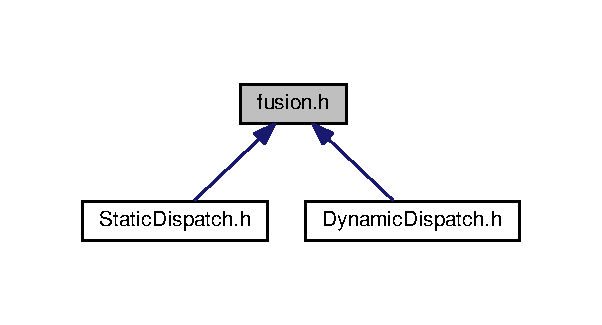
\includegraphics[width=289pt]{fusion_8h__dep__incl}
\end{center}
\end{figure}
\subsection*{Classes}
\begin{DoxyCompactItemize}
\item 
struct \hyperlink{structbuffer__t}{buffer\-\_\-t}
\end{DoxyCompactItemize}
\subsection*{Namespaces}
\begin{DoxyCompactItemize}
\item 
\hyperlink{namespace_fusion}{Fusion}
\end{DoxyCompactItemize}
\subsection*{Macros}
\begin{DoxyCompactItemize}
\item 
\#define \hyperlink{fusion_8h_a2bca21209e0c048138ca68de82240740}{W\-O\-R\-K\-L\-O\-A\-D\-\_\-\-T\-H\-R\-E\-S\-H\-O\-U\-L\-D}~1.\-0
\item 
\#define \hyperlink{fusion_8h_aa482ffee6eeb009f59fa394d256191aa}{fusion\-\_\-printf}(...)~printf(\char`\"{}\%s\textbackslash{}n\char`\"{},\-\_\-\-\_\-\-V\-A\-\_\-\-A\-R\-G\-S\-\_\-\-\_\- );
\item 
\#define \hyperlink{fusion_8h_addf06f0401b4fbc53e7097b4fd536a8b}{F\-U\-S\-I\-O\-N\-\_\-\-H}
\end{DoxyCompactItemize}
\subsection*{Typedefs}
\begin{DoxyCompactItemize}
\item 
typedef struct \hyperlink{structbuffer__t}{buffer\-\_\-t} \hyperlink{fusion_8h_aebe399a52d3e6b4c16909f8216198044}{buffer\-\_\-t}
\end{DoxyCompactItemize}
\subsection*{Functions}
\begin{DoxyCompactItemize}
\item 
int \hyperlink{fusion_8h_a698f0ce388c5fcbbc63ecb696e5b4b97}{halide\-\_\-copy\-\_\-to\-\_\-host} (void $\ast$user\-\_\-context, \hyperlink{structbuffer__t}{buffer\-\_\-t} $\ast$buf)
\end{DoxyCompactItemize}


\subsection{Macro Definition Documentation}
\hypertarget{fusion_8h_addf06f0401b4fbc53e7097b4fd536a8b}{\index{fusion.\-h@{fusion.\-h}!F\-U\-S\-I\-O\-N\-\_\-\-H@{F\-U\-S\-I\-O\-N\-\_\-\-H}}
\index{F\-U\-S\-I\-O\-N\-\_\-\-H@{F\-U\-S\-I\-O\-N\-\_\-\-H}!fusion.h@{fusion.\-h}}
\subsubsection[{F\-U\-S\-I\-O\-N\-\_\-\-H}]{\setlength{\rightskip}{0pt plus 5cm}\#define F\-U\-S\-I\-O\-N\-\_\-\-H}}\label{fusion_8h_addf06f0401b4fbc53e7097b4fd536a8b}
\hypertarget{fusion_8h_aa482ffee6eeb009f59fa394d256191aa}{\index{fusion.\-h@{fusion.\-h}!fusion\-\_\-printf@{fusion\-\_\-printf}}
\index{fusion\-\_\-printf@{fusion\-\_\-printf}!fusion.h@{fusion.\-h}}
\subsubsection[{fusion\-\_\-printf}]{\setlength{\rightskip}{0pt plus 5cm}\#define fusion\-\_\-printf(
\begin{DoxyParamCaption}
\item[{}]{...}
\end{DoxyParamCaption}
)~printf(\char`\"{}\%s\textbackslash{}n\char`\"{},\-\_\-\-\_\-\-V\-A\-\_\-\-A\-R\-G\-S\-\_\-\-\_\- );}}\label{fusion_8h_aa482ffee6eeb009f59fa394d256191aa}
\hypertarget{fusion_8h_a2bca21209e0c048138ca68de82240740}{\index{fusion.\-h@{fusion.\-h}!W\-O\-R\-K\-L\-O\-A\-D\-\_\-\-T\-H\-R\-E\-S\-H\-O\-U\-L\-D@{W\-O\-R\-K\-L\-O\-A\-D\-\_\-\-T\-H\-R\-E\-S\-H\-O\-U\-L\-D}}
\index{W\-O\-R\-K\-L\-O\-A\-D\-\_\-\-T\-H\-R\-E\-S\-H\-O\-U\-L\-D@{W\-O\-R\-K\-L\-O\-A\-D\-\_\-\-T\-H\-R\-E\-S\-H\-O\-U\-L\-D}!fusion.h@{fusion.\-h}}
\subsubsection[{W\-O\-R\-K\-L\-O\-A\-D\-\_\-\-T\-H\-R\-E\-S\-H\-O\-U\-L\-D}]{\setlength{\rightskip}{0pt plus 5cm}\#define W\-O\-R\-K\-L\-O\-A\-D\-\_\-\-T\-H\-R\-E\-S\-H\-O\-U\-L\-D~1.\-0}}\label{fusion_8h_a2bca21209e0c048138ca68de82240740}


\subsection{Typedef Documentation}
\hypertarget{fusion_8h_aebe399a52d3e6b4c16909f8216198044}{\index{fusion.\-h@{fusion.\-h}!buffer\-\_\-t@{buffer\-\_\-t}}
\index{buffer\-\_\-t@{buffer\-\_\-t}!fusion.h@{fusion.\-h}}
\subsubsection[{buffer\-\_\-t}]{\setlength{\rightskip}{0pt plus 5cm}typedef struct {\bf buffer\-\_\-t}  {\bf buffer\-\_\-t}}}\label{fusion_8h_aebe399a52d3e6b4c16909f8216198044}


\subsection{Function Documentation}
\hypertarget{fusion_8h_a698f0ce388c5fcbbc63ecb696e5b4b97}{\index{fusion.\-h@{fusion.\-h}!halide\-\_\-copy\-\_\-to\-\_\-host@{halide\-\_\-copy\-\_\-to\-\_\-host}}
\index{halide\-\_\-copy\-\_\-to\-\_\-host@{halide\-\_\-copy\-\_\-to\-\_\-host}!fusion.h@{fusion.\-h}}
\subsubsection[{halide\-\_\-copy\-\_\-to\-\_\-host}]{\setlength{\rightskip}{0pt plus 5cm}int halide\-\_\-copy\-\_\-to\-\_\-host (
\begin{DoxyParamCaption}
\item[{void $\ast$}]{user\-\_\-context, }
\item[{{\bf buffer\-\_\-t} $\ast$}]{buf}
\end{DoxyParamCaption}
)}}\label{fusion_8h_a698f0ce388c5fcbbc63ecb696e5b4b97}

\hypertarget{fusion__info_8h}{\section{fusion\-\_\-info.\-h File Reference}
\label{fusion__info_8h}\index{fusion\-\_\-info.\-h@{fusion\-\_\-info.\-h}}
}
This graph shows which files directly or indirectly include this file\-:
\nopagebreak
\begin{figure}[H]
\begin{center}
\leavevmode
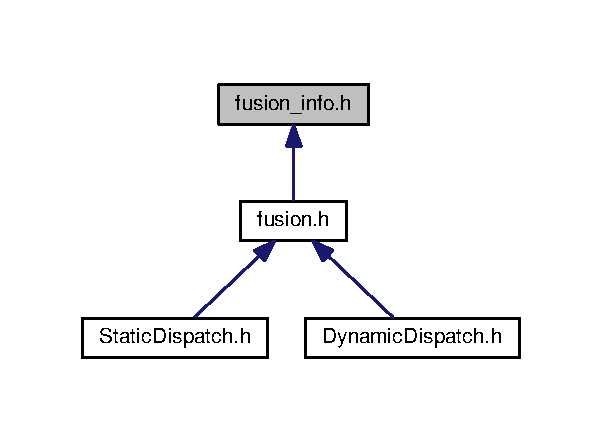
\includegraphics[width=289pt]{fusion__info_8h__dep__incl}
\end{center}
\end{figure}
\subsection*{Enumerations}
\begin{DoxyCompactItemize}
\item 
enum \hyperlink{fusion__info_8h_a015eb90e0de9f16e87bd149d4b9ce959}{status} \{ \hyperlink{fusion__info_8h_a015eb90e0de9f16e87bd149d4b9ce959a0e9a37114c0e458d28d52f06ec0f2242}{idle} =0, 
\hyperlink{fusion__info_8h_a015eb90e0de9f16e87bd149d4b9ce959a71247ee44854ad1f62961a3f25459898}{computing}, 
\hyperlink{fusion__info_8h_a015eb90e0de9f16e87bd149d4b9ce959a23a392e30a43487b88fa5417fdd1d1b2}{writing}, 
\hyperlink{fusion__info_8h_a015eb90e0de9f16e87bd149d4b9ce959aaf38e35232eb6728664f98c8110d11a4}{finished}
 \}
\end{DoxyCompactItemize}


\subsection{Enumeration Type Documentation}
\hypertarget{fusion__info_8h_a015eb90e0de9f16e87bd149d4b9ce959}{\index{fusion\-\_\-info.\-h@{fusion\-\_\-info.\-h}!status@{status}}
\index{status@{status}!fusion_info.h@{fusion\-\_\-info.\-h}}
\subsubsection[{status}]{\setlength{\rightskip}{0pt plus 5cm}enum {\bf status}}}\label{fusion__info_8h_a015eb90e0de9f16e87bd149d4b9ce959}
\begin{Desc}
\item[Enumerator]\par
\begin{description}
\index{idle@{idle}!fusion\-\_\-info.\-h@{fusion\-\_\-info.\-h}}\index{fusion\-\_\-info.\-h@{fusion\-\_\-info.\-h}!idle@{idle}}\item[{\em 
\hypertarget{fusion__info_8h_a015eb90e0de9f16e87bd149d4b9ce959a0e9a37114c0e458d28d52f06ec0f2242}{idle}\label{fusion__info_8h_a015eb90e0de9f16e87bd149d4b9ce959a0e9a37114c0e458d28d52f06ec0f2242}
}]\index{computing@{computing}!fusion\-\_\-info.\-h@{fusion\-\_\-info.\-h}}\index{fusion\-\_\-info.\-h@{fusion\-\_\-info.\-h}!computing@{computing}}\item[{\em 
\hypertarget{fusion__info_8h_a015eb90e0de9f16e87bd149d4b9ce959a71247ee44854ad1f62961a3f25459898}{computing}\label{fusion__info_8h_a015eb90e0de9f16e87bd149d4b9ce959a71247ee44854ad1f62961a3f25459898}
}]\index{writing@{writing}!fusion\-\_\-info.\-h@{fusion\-\_\-info.\-h}}\index{fusion\-\_\-info.\-h@{fusion\-\_\-info.\-h}!writing@{writing}}\item[{\em 
\hypertarget{fusion__info_8h_a015eb90e0de9f16e87bd149d4b9ce959a23a392e30a43487b88fa5417fdd1d1b2}{writing}\label{fusion__info_8h_a015eb90e0de9f16e87bd149d4b9ce959a23a392e30a43487b88fa5417fdd1d1b2}
}]\index{finished@{finished}!fusion\-\_\-info.\-h@{fusion\-\_\-info.\-h}}\index{fusion\-\_\-info.\-h@{fusion\-\_\-info.\-h}!finished@{finished}}\item[{\em 
\hypertarget{fusion__info_8h_a015eb90e0de9f16e87bd149d4b9ce959aaf38e35232eb6728664f98c8110d11a4}{finished}\label{fusion__info_8h_a015eb90e0de9f16e87bd149d4b9ce959aaf38e35232eb6728664f98c8110d11a4}
}]\end{description}
\end{Desc}

\hypertarget{internal_8h}{\section{internal.\-h File Reference}
\label{internal_8h}\index{internal.\-h@{internal.\-h}}
}
{\ttfamily \#include $<$stdint.\-h$>$}\\*
Include dependency graph for internal.\-h\-:
\nopagebreak
\begin{figure}[H]
\begin{center}
\leavevmode
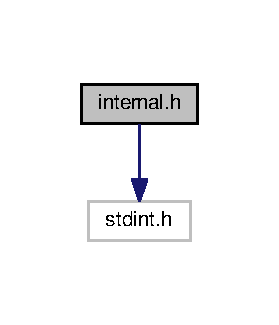
\includegraphics[width=134pt]{internal_8h__incl}
\end{center}
\end{figure}
This graph shows which files directly or indirectly include this file\-:
\nopagebreak
\begin{figure}[H]
\begin{center}
\leavevmode
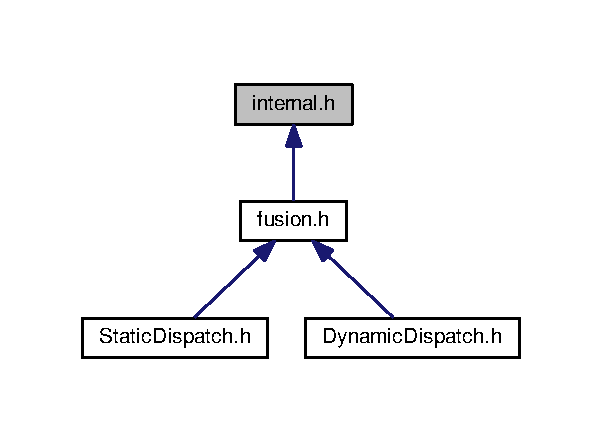
\includegraphics[width=289pt]{internal_8h__dep__incl}
\end{center}
\end{figure}
\subsection*{Classes}
\begin{DoxyCompactItemize}
\item 
struct \hyperlink{structbuffer__t}{buffer\-\_\-t}
\end{DoxyCompactItemize}
\subsection*{Namespaces}
\begin{DoxyCompactItemize}
\item 
\hyperlink{namespace_fusion}{Fusion}
\item 
\hyperlink{namespace_fusion_1_1_internal}{Fusion\-::\-Internal}
\end{DoxyCompactItemize}
\subsection*{Macros}
\begin{DoxyCompactItemize}
\item 
\#define \hyperlink{internal_8h_a8efe382d749baa2b8032e3e844bc6acf}{T\-O\-O\-L\-\_\-\-H}
\end{DoxyCompactItemize}
\subsection*{Typedefs}
\begin{DoxyCompactItemize}
\item 
typedef struct \hyperlink{structbuffer__t}{buffer\-\_\-t} \hyperlink{internal_8h_aebe399a52d3e6b4c16909f8216198044}{buffer\-\_\-t}
\end{DoxyCompactItemize}
\subsection*{Functions}
\begin{DoxyCompactItemize}
\item 
\hyperlink{structbuffer__t}{buffer\-\_\-t} $\ast$ \hyperlink{namespace_fusion_1_1_internal_afa225bde679af6d7984014f0138aa97d}{Fusion\-::\-Internal\-::div\-Buffer} (\hyperlink{structbuffer__t}{buffer\-\_\-t} $\ast$buf, int start, int nend)
\item 
uint8\-\_\-t $\ast$ \hyperlink{namespace_fusion_1_1_internal_a6e60ee6f87aefcec5b810c52ec9d4abb}{Fusion\-::\-Internal\-::init\-Buffer\-\_\-t} (int x, int y, int z, int w, \hyperlink{structbuffer__t}{buffer\-\_\-t} $\ast$buf, int bit\-Of\-Input)
\end{DoxyCompactItemize}


\subsection{Macro Definition Documentation}
\hypertarget{internal_8h_a8efe382d749baa2b8032e3e844bc6acf}{\index{internal.\-h@{internal.\-h}!T\-O\-O\-L\-\_\-\-H@{T\-O\-O\-L\-\_\-\-H}}
\index{T\-O\-O\-L\-\_\-\-H@{T\-O\-O\-L\-\_\-\-H}!internal.h@{internal.\-h}}
\subsubsection[{T\-O\-O\-L\-\_\-\-H}]{\setlength{\rightskip}{0pt plus 5cm}\#define T\-O\-O\-L\-\_\-\-H}}\label{internal_8h_a8efe382d749baa2b8032e3e844bc6acf}


\subsection{Typedef Documentation}
\hypertarget{internal_8h_aebe399a52d3e6b4c16909f8216198044}{\index{internal.\-h@{internal.\-h}!buffer\-\_\-t@{buffer\-\_\-t}}
\index{buffer\-\_\-t@{buffer\-\_\-t}!internal.h@{internal.\-h}}
\subsubsection[{buffer\-\_\-t}]{\setlength{\rightskip}{0pt plus 5cm}typedef struct {\bf buffer\-\_\-t}  {\bf buffer\-\_\-t}}}\label{internal_8h_aebe399a52d3e6b4c16909f8216198044}

\hypertarget{_static_dispatch_8h}{\section{Static\-Dispatch.\-h File Reference}
\label{_static_dispatch_8h}\index{Static\-Dispatch.\-h@{Static\-Dispatch.\-h}}
}
{\ttfamily \#include \char`\"{}clock.\-h\char`\"{}}\\*
{\ttfamily \#include \char`\"{}fusion.\-h\char`\"{}}\\*
Include dependency graph for Static\-Dispatch.\-h\-:
\nopagebreak
\begin{figure}[H]
\begin{center}
\leavevmode
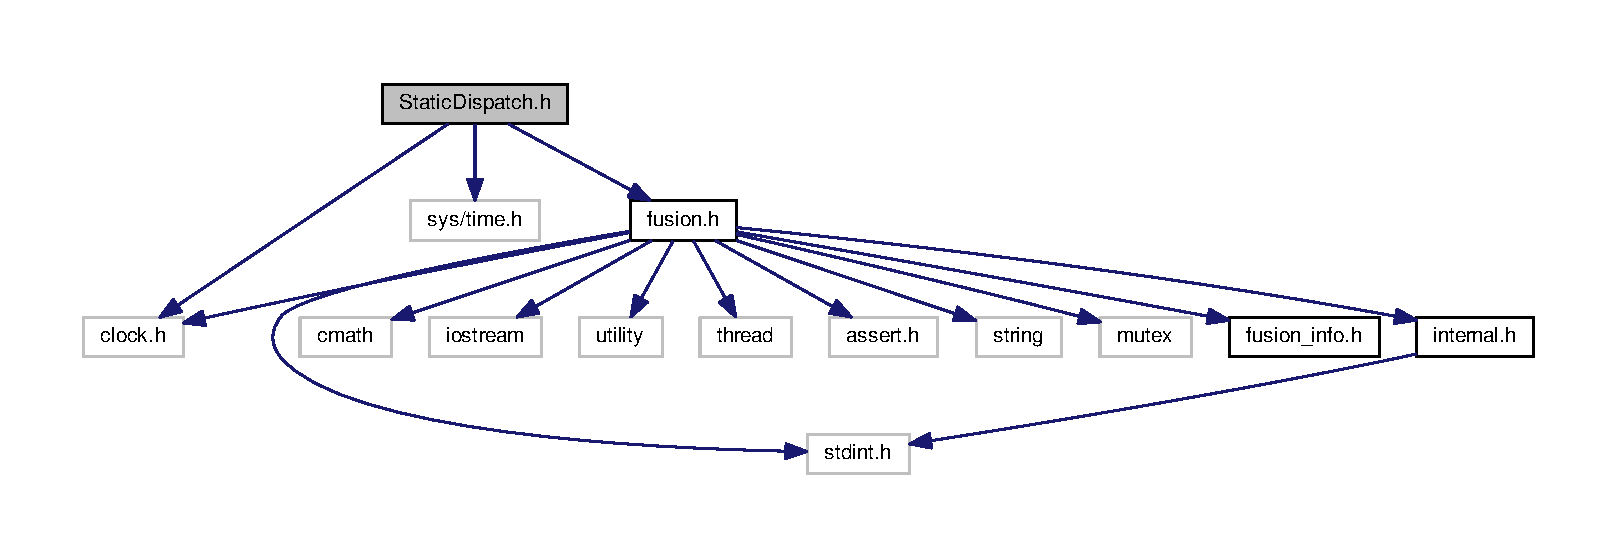
\includegraphics[width=350pt]{_static_dispatch_8h__incl}
\end{center}
\end{figure}
\subsection*{Classes}
\begin{DoxyCompactItemize}
\item 
class \hyperlink{class_fusion_1_1_static_1_1_static_dispatch}{Fusion\-::\-Static\-::\-Static\-Dispatch$<$ Args $>$}
\end{DoxyCompactItemize}
\subsection*{Namespaces}
\begin{DoxyCompactItemize}
\item 
\hyperlink{namespace_fusion}{Fusion}
\item 
\hyperlink{namespace_fusion_1_1_static}{Fusion\-::\-Static}
\end{DoxyCompactItemize}
\subsection*{Functions}
\begin{DoxyCompactItemize}
\item 
{\footnotesize template$<$typename... Args$>$ }\\void \hyperlink{namespace_fusion_1_1_static_a4dda28311f1977091df5d7adb5aec742}{Fusion\-::\-Static\-::gpu\-Stealing} (Args...\-args, function$<$ int(Args..., \hyperlink{structbuffer__t}{buffer\-\_\-t} $\ast$, \hyperlink{structbuffer__t}{buffer\-\_\-t} $\ast$)$>$ func, \hyperlink{structbuffer__t}{buffer\-\_\-t} $\ast$input, \hyperlink{structbuffer__t}{buffer\-\_\-t} $\ast$cpu\-Buf, \hyperlink{structbuffer__t}{buffer\-\_\-t} $\ast$gpu\-Buf, \hyperlink{fusion__info_8h_a015eb90e0de9f16e87bd149d4b9ce959}{status} table\mbox{[}$\,$\mbox{]}, int offset, mutex $\ast$table\-\_\-mutex)
\begin{DoxyCompactList}\small\item\em This Function is a thread function for \hyperlink{namespace_fusion_1_1_static}{Static} execution way with Stealing. \end{DoxyCompactList}\item 
{\footnotesize template$<$typename... Args$>$ }\\void \hyperlink{namespace_fusion_1_1_static_a36302361627ccb126b6aeb0efa6d3ab2}{Fusion\-::\-Static\-::gpu\-Thread} (Args...\-args, function$<$ int(Args..., \hyperlink{structbuffer__t}{buffer\-\_\-t} $\ast$, \hyperlink{structbuffer__t}{buffer\-\_\-t} $\ast$)$>$ func, \hyperlink{structbuffer__t}{buffer\-\_\-t} $\ast$input, \hyperlink{structbuffer__t}{buffer\-\_\-t} $\ast$output)
\end{DoxyCompactItemize}

%--- End generated contents ---

% Index
\newpage
\phantomsection
\addcontentsline{toc}{chapter}{Index}
\printindex

\end{document}
